%% abtex2-modelo-trabalho-academico.tex, v-1.9.3 laurocesar
%% Copyright 2012-2015 by abnTeX2 group at http://abntex2.googlecode.com/ 
%% This work may be distributed and/or modified under the
%% conditions of the LaTeX Project Public License, either version 1.3
%% of this license or (at your option) any later version.
%% The latest version of this license is in
%%   http://www.latex-project.org/lppl.txt
%% and version 1.3 or later is part of all distributions of LaTeX
%% version 2005/12/01 or later.
%%
%% This work has the LPPL maintenance status `maintained'.
%% 
%% The Current Maintainer of this work is the abnTeX2 team, led
%% by Lauro César Araujo. Further information are available on 
%% http://abntex2.googlecode.com/
%%
%% This work consists of the files abntex2-modelo-trabalho-academico.tex,
%% abntex2-modelo-include-comandos and abntex2-modelo-references.bib
%%

% ------------------------------------------------------------------------
% ------------------------------------------------------------------------
% abnTeX2: Modelo de Trabalho Academico (tese de doutorado, dissertacao de
% mestrado e trabalhos monograficos em geral) em conformidade com 
% ABNT NBR 14724:2011: Informacao e documentacao - Trabalhos academicos -
% Apresentacao
% ------------------------------------------------------------------------
% ------------------------------------------------------------------------

\documentclass[
	% -- opções da classe memoir --
	12pt,				% tamanho da fonte
	openright,			% capítulos começam em pág ímpar (insere página vazia caso preciso)
	twoside,			% para impressão em verso e anverso. Oposto a oneside
	a4paper,			% tamanho do papel. 
	% -- opções da classe abntex2 --
	%chapter=TITLE,		% títulos de capítulos convertidos em letras maiúsculas
	%section=TITLE,		% títulos de seções convertidos em letras maiúsculas
	%subsection=TITLE,	% títulos de subseções convertidos em letras maiúsculas
	%subsubsection=TITLE,% títulos de subsubseções convertidos em letras maiúsculas
	% -- opções do pacote babel --
	english,			% idioma adicional para hifenização
	brazil				% o último idioma é o principal do documento
	]{abntex2}

% ---
% Pacotes básicos 
% ---
% \usepackage{uarial}				% Usa a fonte Latin Modern			lmodern
\usepackage[T1]{fontenc}		% Selecao de codigos de fonte.
\usepackage[utf8]{inputenc}		% Codificacao do documento (conversão automática dos acentos)
\usepackage{lastpage}			% Usado pela Ficha catalográfica
\usepackage{indentfirst}		% Indenta o primeiro parágrafo de cada seção.
\usepackage{color}				% Controle das cores
\usepackage{graphicx}			% Inclusão de gráficos
\usepackage{microtype} 			% para melhorias de justificação

% pacotes adicionados
\usepackage{amsmath}
\usepackage{amssymb,amsfonts,amsthm}
\usepackage{setspace}

\usepackage[utf8]{inputenc}
\usepackage[T1]{fontenc}

% ---
		
% ---
% Pacotes adicionais, usados apenas no âmbito do Modelo Canônico do abnteX2
% ---
\usepackage{lipsum}				% para geração de dummy text
% ---
\usepackage{todonotes}
% ---
% Pacotes de citações
% ---
\usepackage[brazilian,hyperpageref]{backref}	 % Paginas com as citações na bibl
\usepackage[alf]{abntex2cite}	% Citações padrão ABNT


\renewcommand{\bf}[1]{\mathbf{#1}}
\renewcommand{\rm}[1]{\mathrm{#1}}

\usepackage{graphicx}
\usepackage{subfig}

\usepackage{cite}
\renewcommand\citeleft{[}
\renewcommand\citeright{]}

% --- 
% CONFIGURAÇÕES DE PACOTES
% --- 
\renewcommand{\imprimircapa}{
\thispagestyle{empty}

\vfill
 \begin{center}
    
    \begin{figure}
	   \centering
	   		
\includegraphics[scale=0.35]{figs/brasao_uesc.png} 
    \end{figure}
    
    {\large\bfseries UNIVERSIDADE ESTADUAL DE SANTA CRUZ} \\
    
   
    % {\large\bfseries CAMPUS Prof. SOANE NAZARÉ DE ANDRADE}  \\ 

    \vspace*{1in}
    \begin{large} \bfseries THALES AUGUSTO RAMOS VIEIRA \end{large}\\[0.4in]

    \vspace*{4cm}
    \noindent \\
    
    \large\bfseries{\begin{large}ABORDAGEM DE UM SISTEMA WEB PARA FACILITAR A MERCANCIA NO AMBIENTE UNIVERSITÁRIO \end{large}} \\
    \vfill
    \large\bfseries{ ILHÉUS - BAHIA \\ 2020}
\end{center}

\normalsize


}


\renewcommand{\imprimirfolhaderosto}{

\begin{center}

    {\large \begin{large} \bfseries THALES AUGUSTO RAMOS VIEIRA \end{large}\\}
    \vspace{8cm}
    {\large\bfseries{\begin{large}ABORDAGEM DE UM SISTEMA WEB PARA FACILITAR A MERCANCIA NO AMBIENTE UNIVERSITÁRIO \end{large}}\\}
    \vspace{1cm}
    \hspace{.45\linewidth}
    \begin{minipage}{.50\linewidth}

    Trabalho de Conclusão de Curso submetido à Universidade Estadual de Santa Cruz como requisito para obtenção do grau de Bacharel em Ciência de Computação. 

            \textbf{\\ Orientador: Prof Hélder Conceição Almeida}
           
    
    \end{minipage}

    \vspace{2cm}
    \vfill
    {\large\bfseries{ ILHÉUS - BAHIA \\ 2019}}
\end{center}

}


% ---
% Configurações do pacote backref
% Usado sem a opção hyperpageref de backref
\renewcommand{\backrefpagesname}{Citado na(s) página(s):~}
% Texto padrão antes do número das páginas
\renewcommand{\backref}{}
% Define os textos da citação
\renewcommand*{\backrefalt}[4]{
	\ifcase #1 %
		Nenhuma citação no texto.%
	\or
		Citado na página #2.%
	\else
		Citado #1 vezes nas páginas #2.%
	\fi}%
% ---
% ---
% Informações de dados para CAPA e FOLHA DE ROSTO
% ---

\titulo{Abordagem de um sistema web para facilitar o fluxo de compra e venda no ambiente universitário}
\autor{Thales Augusto Ramos Vieira}
\local{Brasil}
\data{2019, v-1.0.0}
\orientador{Hélder Conceição Almeida}
%\coorientador{coorientador}
\instituicao{%
  Universidade Estadual de Santa Cruz
  \par
  Departamento de Ciências Exatas e Tecnológicas
  }
\tipotrabalho{Projeto de Fim de Curso}
% O preambulo deve conter o tipo do trabalho, o objetivo, 
% o nome da instituição e a área de concentração 
\preambulo{O preambulo deve conter o tipo do trabalho, o objetivo, o nome da instituição e a área de concentração }
% ---






% ---
% Configurações de aparência do PDF final

% alterando o aspecto da cor azul
\definecolor{blue}{RGB}{41,5,195}

% informações do PDF
\makeatletter
\hypersetup{
     	%pagebackref=true,
		colorlinks=true,       		% false: boxed links; true: colored links
    	linkcolor=blue,          	% color of internal links
    	citecolor=black,        		% color of links to bibliography
    	filecolor=magenta,      		% color of file links
		urlcolor=blue,
		bookmarksdepth=4
}



\makeatother
% --- 

% --- 
% Espaçamentos entre linhas e parágrafos 
% --- 

% O tamanho do parágrafo é dado por:
\setlength{\parindent}{1.3cm}

% Controle do espaçamento entre um parágrafo e outro:
\setlength{\parskip}{0.2cm}  % tente também \onelineskip

% ---
% compila o indice
% ---
\makeindex
% ---

% ----
% Início do documento
% ----
\usepackage{float}
\begin{document}

% Seleciona o idioma do documento (conforme pacotes do babel)
%\selectlanguage{english}
\selectlanguage{brazil}

% Retira espaço extra obsoleto entre as frases.
\frenchspacing 

% ----------------------------------------------------------
% ELEMENTOS PRÉ-TEXTUAIS
% ----------------------------------------------------------
\pretextual

% ---
% Capa
% ---
\imprimircapa
% ---

% ---
% Folha de rosto
% (o * indica que haverá a ficha bibliográfica)
% ---
\imprimirfolhaderosto

% ---
% Inserir a ficha bibliografica
% ---

% Isto é um exemplo de Ficha Catalográfica, ou ``Dados internacionais de
% catalogação-na-publicação''. Você pode utilizar este modelo como referência. 
% Porém, provavelmente a biblioteca da sua universidade lhe fornecerá um PDF
% com a ficha catalográfica definitiva após a defesa do trabalho. Quando estiver
% com o documento, salve-o como PDF no diretório do seu projeto e substitua todo
% o conteúdo de implementação deste arquivo pelo comando abaixo:
%
% \begin{fichacatalografica}
%     \includepdf{fig_ficha_catalografica.pdf}
% \end{fichacatalografica}

\begin{fichacatalografica}
%	\sffamily
%	\vspace*{\fill}					% Posição vertical
%	\begin{center}					% Minipage Centralizado
%	\fbox{\begin{minipage}[c][8cm]{13.5cm}		% Largura
%	\small
%	\imprimirautor
%	%Sobrenome, Nome do autor
%	
%	\hspace{0.5cm} \imprimirtitulo  / \imprimirautor. --
%	\imprimirlocal, \imprimirdata-
%	
%	\hspace{0.5cm} \pageref{LastPage} p. : il. (algumas color.) ; 30 cm.\\
%	
%	\hspace{0.5cm} \imprimirorientadorRotulo~\imprimirorientador\\
%	
%	\hspace{0.5cm}
%	\parbox[t]{\textwidth}{\imprimirtipotrabalho~--~\imprimirinstituicao,
%	\imprimirdata.}\\
%	
%	\hspace{0.5cm}
%		1. Palavra-chave1.
%		2. Palavra-chave2.
%		2. Palavra-chave3.
%		I. Orientador.
%		II. Universidade xxx.
%		III. Faculdade de xxx.
%		IV. Título 			
%	\end{minipage}}
%	\end{center}
\end{fichacatalografica}
%% ---
% Inserir errata
% ---
\begin{errata}
Elemento opcional da \citeonline[4.2.1.2]{NBR14724:2011}. Exemplo:

\vspace{\onelineskip}

FERRIGNO, C. R. A. \textbf{Tratamento de neoplasias ósseas apendiculares com
reimplantação de enxerto ósseo autólogo autoclavado associado ao plasma
rico em plaquetas}: estudo crítico na cirurgia de preservação de membro em
cães. 2011. 128 f. Tese (Livre-Docência) - Faculdade de Medicina Veterinária e
Zootecnia, Universidade de São Paulo, São Paulo, 2011.

\begin{table}[htb]
\center
\footnotesize
\begin{tabular}{|p{1.4cm}|p{1cm}|p{3cm}|p{3cm}|}
  \hline
   \textbf{Folha} & \textbf{Linha}  & \textbf{Onde se lê}  & \textbf{Leia-se}  \\
    \hline
    1 & 10 & auto-conclavo & autoconclavo\\
   \hline
\end{tabular}
\end{table}

\end{errata}
% ---

% ---
% Inserir folha de aprovação
% ---

% Isto é um exemplo de Folha de aprovação, elemento obrigatório da NBR
% 14724/2011 (seção 4.2.1.3). Você pode utilizar este modelo até a aprovação
% do trabalho. Após isso, substitua todo o conteúdo deste arquivo por uma
% imagem da página assinada pela banca com o comando abaixo:
%
% \includepdf{folhadeaprovacao_final.pdf}
%
\begin{folhadeaprovacao}


\begin{center}
    % Novo

    {\large \begin{large} \bfseries THALES AUGUSTO RAMOS VIEIRA \end{large}\\}
    \vspace{4cm}
    {\large\bfseries{\begin{large}ABORDAGEM DE UM SISTEMA WEB PARA FACILITAR A MERCÂNCIA NO AMBIENTE UNIVERSITÁRIO \end{large}}\\}
    \vspace{1cm}
    \hspace{.45\linewidth}
    \begin{minipage}{.50\linewidth}

            \textbf{Trabalho de Conclusão de Curso submetido à Universidade Estadual de Santa Cruz  como requisito 
            para obtenção do grau de Bacharel em Ciência de Computação. }
    \end{minipage}
    \\
\end{center}
    \textbf{Ilhéus, xx de julho de 2019.}
\begin{center}
            % {UNIVERSIDADE ESTADUAL DE SANTA CRUZ} \\
           

    % \vspace{1.5cm}
    %                                 {\begin{large} \bfseries PATRICK SILVA FERRAZ \end{large}}\\
    \bfseries{}
\end{center}

% Esta Monografia foi julgada adequada, como requisito parcial, para a obten\c{c}\~{a}o do título  de Bacharel em Ciência de Computação, sendo aprovada em sua forma final  pela banca examinadora:

    \vspace{2.5cm}
    \assinatura{Orientador(a): Prof. Me. Hélder Conceição Almeida \\ Universidade Estadual de Santa Cruz}
    \assinatura{Prof. Dr. Marcelo Ossamu Honda \\ Universidade Estadual de Santa Cruz}
    \assinatura{Prof. Me. Lília Soussa Marta \\ Universidade Estadual de Santa Cruz}
    \vspace{3 cm}%\vfill

    % \begin{center}
    %     Ilhéus, 06 de julho de 2018
    % \end{center}
  
\end{folhadeaprovacao}
% ---
% Dedicatória
% ---
\begin{dedicatoria}
   \vspace*{\fill}
   \centering
   \noindent
   \textit{ Este trabalho é dedicado a todas as pessoas que tem um sonho.} \vspace*{\fill}
\end{dedicatoria}
% ---
% ---
% Agradecimentos
% ---
\begin{agradecimentos}
Aos meus pais, minha base de tudo, sempre me ensinaram a ser uma pessoa digna e batalhadora, busquei inspiração neles para ir tão longe, devo tudo a eles.

À meu irmão, por sempre tirar minha paciência e me amar ao mesmo tempo.

À Ricardo e Fabrícia, por ter me dado a incrível oportunidade de dar o ponta pé inicial na minha carreira.

Aos meus parentes, por sempre estar na torcida por mim, celebrando a cada nova conquista na minha vida.

Aos meus amigos de infância, que fizeram parte da minha vida contribuindo para eu me tornar quem sou.

Aos meus amigos da UESC, que sempre me motivaram a vencer a graduação e crescer na vida.

Aos professores e funcionários, por transmitir seus conhecimentos durantes esses anos de graduação.

À CNPq por corroborar com minhas pesquisas científicas por meio de bolsas.

À NBCGIB por fornecer um lugar colaborativo e adequado para o meu crescimento intelectual.

À Techmobil, por acreditar no meu conhecimento técnico e por fornecer um ótimo ambiente de trabalho.

Aos bares do Salobrinho, por me vender muita cerveja e ter me proporcionado momentos inesquecíveis.

\end{agradecimentos}
% ---
% ---
% Epígrafe
% ---
\begin{epigrafe}
    \vspace*{\fill}
	\begin{flushright}
\textit{ Não sabendo que era impossível, foi lá e fez ...\\ Jean Cocteau}
	\end{flushright}
\end{epigrafe}
% ---

% ---
% RESUMOS
% ---

% resumo em português
\setlength{\absparsep}{18pt} % ajusta o espaçamento dos parágrafos do resumo
\begin{resumo}
Lorem ipsum dolor sit amet, consectetur adipiscing elit. Morbi eleifend rutrum ligula, a pharetra libero dictum vitae. Duis id mauris erat. Nunc eu efficitur tortor. Praesent volutpat quis quam vel condimentum. Pellentesque augue leo, volutpat a orci non, fermentum malesuada mi. In eget mollis enim. In pharetra facilisis leo id placerat. Aliquam consequat molestie nisi ac convallis. Proin ut augue non tellus efficitur egestas sed vitae eros. Aenean ac mauris vel ante rutrum hendrerit ut non nibh. Pellentesque lacus felis, volutpat nec vulputate id, interdum id nunc. In molestie scelerisque ultrices. Etiam ac nisi eros. Vivamus arcu mi, iaculis id est ac, volutpat aliquet purus. Donec tincidunt nibh quis justo tristique porttitor. In odio dolor, viverra aliquet tempus egestas, pellentesque sed ante. Donec tempus libero sit amet ante vehicula, ac mollis mi semper. Nunc id tortor blandit, dapibus purus sed, imperdiet lorem. Sed condimentum risus ligula, sit amet accumsan diam tempus quis. Curabitur ultricies in nisi ut laoreet. Phasellus volutpat, risus et commodo volutpat, ex purus efficitur eros, in pulvinar lorem sem quis mi. Nulla tristique commodo elit, ac pulvinar nisi tempus quis. In iaculis, dui a aliquet vestibulum, neque ligula facilisis nisi, ac porta ligula enim non metus. Vivamus accumsan dolor in lorem aliquet molestie. In ac dolor elit. Morbi mollis tortor a ligula blandit mollis. Nulla dignissim elementum est, a porttitor ante faucibus quis. Vestibulum ultricies risus quis egestas volutpat. Mauris accumsan ut dolor vitae consequat. Nam eleifend mauris sapien, sit amet tempor enim condimentum vel. Maecenas dictum ultricies turpis eget commodo. Aenean tristique, purus quis pulvinar dignissim, tellus leo gravida augue, quis pellentesque nunc elit et risus. Donec egestas nibh ut nisi molestie, sit amet ultricies nunc sollicitudin. Proin consectetur leo et sapien imperdiet accumsan. Morbi mattis ante et risus lobortis varius quis in ipsum. Duis dignissim porttitor diam, vel maximus tortor luctus sed. Vivamus eget ipsum imperdiet neque accumsan aliquam vel ut tellus. Pellentesque habitant morbi tristique senectus et netus et malesuada fames ac turpis egestas. In scelerisque erat ligula, non gravida urna interdum eget. Donec iaculis, lacus rutrum porttitor venenatis, erat eros tincidunt mi, sit amet varius mi nunc sed nibh. In maximus, neque at interdum tristique, sapien metus condimentum nunc, eget convallis urna nibh sit amet lectus. Duis at malesuada libero. Morbi ullamcorper purus at imperdiet lobortis. Nullam ante purus, lacinia ac porttitor ultricies, egestas vitae neque. Morbi malesuada, tellus et aliquet sodales, metus mauris ultrices purus, sed ultrices metus mauris mattis nunc. Praesent finibus semper dapibus. Nam rhoncus ante ac felis tristique convallis. Pellentesque a mauris vitae ligula mattis vulputate faucibus in purus. Sed molestie purus massa, at bibendum urna suscipit non. Nam dui turpis, ullamcorper nec mauris imperdiet, blandit elementum augue. Proin ullamcorper, nibh ac tempor dictum, quam felis varius dolor, a feugiat nisi massa et lorem. Mauris eget tortor elit. Phasellus rutrum turpis ipsum, at mattis urna tempus at. Ut turpis purus, semper ut enim sit amet, blandit scelerisque erat. Duis at lorem ipsum. Mauris vel imperdiet metus. Suspendisse potenti. Nunc.


 \textbf{Palavras-chave}: sistema web, mercância, universidade.
\end{resumo}

% resumo em inglês
\begin{resumo}[Abstract]
 \begin{otherlanguage*}{english}
 % Realizar a verificação ortográfica, sintaxe e semântica.

   \vspace{\onelineskip}
 
   \noindent 
   \textbf{Keywords}: .
 \end{otherlanguage*}
\end{resumo}

%% resumo em francês 
%\begin{resumo}[Résumé]
% \begin{otherlanguage*}{french}
%    Il s'agit d'un résumé en français.
% 
%   \textbf{Mots-clés}: latex. abntex. publication de textes.
% \end{otherlanguage*}
%\end{resumo}
%
%% resumo em espanhol
%\begin{resumo}[Resumen]
% \begin{otherlanguage*}{spanish}
%   Este es el resumen en español.
%  
%   \textbf{Palabras clave}: latex. abntex. publicación de textos.
% \end{otherlanguage*}
%\end{resumo}
% ---

% ---
% inserir lista de ilustrações
% ---
\pdfbookmark[0]{\listfigurename}{lof}
\listoffigures*
\cleardoublepage
%% ---

% ---
% inserir lista de tabelas
% ---
\pdfbookmark[0]{\listtablename}{lot}
\listoftables*
\cleardoublepage
% ---
% ---
% inserir lista de abreviaturas e siglas
% ---
\begin{siglas}
% \item[ABNT] Associação Brasileira de Normas Técnicas
% \item[API] \textit{Application Programming Interface}
% \item[BGR] \textit{Blue, Green, Red}
% \item[BGRA] \textit{Blue, Green, Red, Alpha}
% \item[CMYK] \textit{Cyan, Magenta, Yellow and Key (Black)}
% \item[ECA] \textit{European Cocoa Association}
% \item[FCC] \textit{Federation of Cocoa Commerce}
% \item[GPU] \textit{Graphics Processing Unit}
% \item[HSV] \textit{Hue, Saturation, Value}
% \item[IDE] \textit{Integrated Development Environment}
% \item[ISO] \textit{International Organization for Standardization}User Experience(UX)Não Relacional(NoSQL)
% Secure Sockets Layer}(SSL
\item[SSL] \textit{Secure Sockets Layer}
% \item[NoSQL] \textit{Não Relacional}
\item[RoR] \textit{Ruby on Rails}
\item[UX] \textit{User Experience}
\item[MVC] \textit{Model-View-Controller}
\item[OSS] \textit{Open Source Software}
\item[ACID] \textit{Atomicidade, Consistência, Isolamento e Durabilidade}
\item[BDD] \textit{Behaviour-Driven Development}
\item[SGBD] \textit{Sistema Gerenciador de Banco de Dados}
% OSS(\textit{Open Source Software})Sistema Gerenciador de Banco de Dados(SGBD)
% \item[NDK] \textit{Native Development Kit}
% \item[OS] \textit{Operational System}
% \item[OODA] Orientar, Observar, Decidir e Agir
% \item[ROI] \textit{Region Of Interest}Atomicidade, Consistência, Isolamento e Durabilidade
% \item[TDD] \textit{Test Driven Development}
% \item[UML] \textit{Unified Modeling Language}
%  É necessário colocar dos operadores lógicos (AND, OR, NOT e XOR?)
%  \item[] \textit{}
%  \item[] \textit{}
%  \item[] \textit{}
\end{siglas}
% ---

% ---
% inserir lista de símbolos
% ---
% \begin{simbolos}
%  \item[$ CO_2 $] Dióxido de Carbono
%  \item[$C_{3+}$] Hidrocarbonetos com três ou mais carbonos
% \end{simbolos}
% ---





% ---
% inserir o sumario
%% ---
\pdfbookmark[0]{\contentsname}{toc}
\tableofcontents*
\cleardoublepage
%% ---



% ----------------------------------------------------------
% ELEMENTOS TEXTUAIS
% ----------------------------------------------------------
\textual

\chapter{Introdução}

% Contextualizar.....

De acordo com os dados de 2018 da OIT\cite{grimshaw2019resumen}, cerca de 61\% dos trabalhadores do mundo atuam de maneira informal, isso equivale a cerca de 2 bilhões de pessoas. Já no Brasil, essa informalidade chega a atingir 41,3\% da população em 2019, segundo dados do IBGE. Do mesmo modo, no ambiente universitário muitos alunos necessitam algum complemento de renda para manter sua permanência e estudos. Dessa forma, optam por vender artefatos, alimentos, colares, roupas, dentre outros produtos para a comunidade acadêmica, bem como seus arredores.

O advento de novas tecnologias da informação consolidou um novo paradigma econômico, sendo possível a criação de novos mercados, o que contribuiu para a venda de produtos e serviços por meio dessa tecnologia. Diante desse novo modelo de mercância, espera-se que o âmbito universitário tire proveito, buscando a aproximar pessoas interessadas a vender de pessoas interessadas a comprar produtos e serviços.

Visto isso, o atual trabalho propõe um meio tecnológico, simples e objetivo para facilitar o processo mercantil informal nas universidades do Brasil.

\section{O problema}

A principal forma utilizada pelos vendedores para divulgação de produtos no ambiente acadêmico é por meio de redes sociais como o Whatsapp, Instagram e Facebook. Porém essas ferramentas descentralizadas, em muitos casos, não alcançam o efeito desejado sobre  o trâmite de compra e venda.

Tal descentralização é ruim para o vendedor, sendo necessário manipular e administrar diversas ferramentas para um mesmo objetivo. Do mesmo modo se apresenta ruim para os clientes, aos quais necessitam ter o número e Instagram de diversos vendedores para realizar a comunicação necessária para realizar as compras. 

Mas, e se esses dados estivessem reunidos em um só lugar? E se fosse possível o acesso ao preço dos produtos de cada vendedor, bem como seus dados de contato? E se fosse possível realizar a devida compra com poucas ações? Esse é o grande problema da descentralização da informação mercantil nas universidades.

\section{Justificativa}
\label{sec:justificativa}

Como será melhor abordado na seção \ref{trabalho_informal}, o principal motivo para evasão universitária são as dificuldades financeiras que os alunos passam. O segundo motivo é a dificuldade de conciliar trabalho e estudo. Diante desses motivos, se faz necessário a elaboração de uma solução que contribua para que a condição financeira do aluno seja melhorada, passando assim a conseguir se manter na universidade e possivelmente não necessitar de trabalhos externos a universidade para que seja possível se manter na mesma.

Através da realização deste projeto, espera-se ampliar a circulação financeira entre os membros da comunidade acadêmica, facilitando, assim, o comércio informal e, consequentemente, melhorando a autonomia financeira do estudante.

\section{Objetivos}

\subsection{Objetivo Geral}

Solucionar o problema apresentado por meio de recursos tecnológicos. Será implementado um sistema web para facilitar esse processo mercantil entre o vendedor e comprador no ambiente acadêmico.

\subsection{Objetivos Específicos}
\begin{enumerate}
    % \item Elaborar uma análise de requisitos para o problema.
    \item Desenvolver um sistema web que solucione o problema
    % \item Aplicar uma metodologia ágil durante o desenvolvimento.
    \item Validar e confiabilizar o sistema por meio de testes automatizados.
    \item Disponibilizar o código fonte da aplicação
    \item Comparar o sistema final com o mockup proposto
    \item Disponibilizar o sistema para a comunidade acadêmica
\end{enumerate}


\section{Organização}
O presente projeto está dividido em 5 capítulos, e organizado da seguinte forma:

No Capítulo II encontra-se o referencial teórico, apresentando todos os fundamentos teóricos que solidificam e criam uma base para o entendimento do trabalho como um todo.

No Capítulo III está explicado toda a metodologia que foi utilizada para chegar ao resultado, mostrando cada passo de forma detalhada.

Os resultados alcançados e discussões serão abordados no Capítulo IV, ao qual será realizado uma comparação com os objetivos que foram propostos.

No Capítulo V será discutida a conclusão acerca do trabalho, bem como apresentar possíveis os trabalhos futuros necessários para uma boa continuação do projeto.
    
% Introduzir Figura
%\begin{figure}
%	   \centering
%	   		\includegraphics[scale=0.35]{figs/MPCbase.PNG} 
%	   \caption{Algoritmo MPC}
%	   \label{label para referencia cruzada Figura}
%\end{figure}


% Lista de Item

%\begin{itemize}
%	\item item 1
%	\item item 2
%	\item item 3
%\end{itemize}

% Equação
%\begin{equation}
%	\label{label para referencia cruzada %equacoes} 
%	y(t)=\sum_{i=1}^{\infty}h_i\Delta u(t-i)
%\end{equation}

% Equação em linha 
%$\hat{y}(t+k\mid t)= \sum^\infty_{i=1} g_i %\Delta u(t+k-i\mid t)$

% Citação -  Criei o arquivo de bibliografia usando o jabref

%\cite{Camacho2007} 

% Referencia Cruzada de Figura
%\ref{label para referencia cruzada Figura}

% Referencia Cruzada de Equação
%\ref{label para referencia cruzada equacoes}


% Tabelas

%\begin{table}[h]
%\begin{center}
%     \caption{Índices 1 para casos factíveis}
%     \begin{tabular}{| l | l | l | l |}
%     \hline Índice & LP Petro & LP 2 & %Diferença\\ 
%     \hline $SES_y$& 60.5406 & 60.5492 & %-0.0087\\
%     \hline $SES_u$& 1166.1464 & 1166.1464 & 2.36*$10^{-9}$ \\
%     \hline
 
%    \end{tabular}
%\label{table:indices1}
%\end{center}
%\end{table}
\chapter{Referencial Teórico}

Essa seção tem como objetivo explicar o funcionamento de um sistema web, conhecimento necessário pois é a base de todo o projeto que aqui será demonstrado. Outros temas importantes serão abordados, como metodologia de desenvolvimento de software e padrões de código. \par
Os tópicos aqui abordados servirão para nortear a metodologia proposta neste trabalho, buscando assim criar uma base sólida para os argumentos que serão apresentados. Alguns trabalhos semelhantes serão apresentados com a intenção de ajudar a contextualizar esse projeto aqui desenvolvido.


\section{Trabalho informal}\label{trabalho_informal}
Não foram encontrados artigos acerca do trabalho informal dentro das universidades, mas iremos usar como base uma pesquisa sobre o trabalho informal de jovens estudantes. Dois motivos para a inserção dos estudantes no mercado de trabalho informal é ajudar na renda familiar e obter independência financeira\cite{ferreira2009trabalhojovem}. \par
De acordo com questionário fechado e entrevistas feitas por \cite{ribeiro2005evasao}, os motivos da evasão geralmente são causados por dificuldades financeiras, vocacionais, educacionais e de dedicação. Dentre as dificuldades citadas, uma se destacou por ser o principal motivo de evasão dos estudantes entrevistado, a dificuldade financeira. Diante disso, o projeto irá atuar consistentemente em um dos motivos de evasão universitária, a dificuldade financeira, buscando assim um meio de sanar tal problema.

\section{Aplicações web}
\label{sec:trabalhos_correlatos}

Na década de 1990 foi concebida uma nova tecnologia para a internet: a Tecnologia Web\cite{zaneti2005construcao}. O advento dessa nova tecnologia ocorreu devido a necessidade de formar um repositório de conhecimento humano \cite{lee1994www} e está baseada em troca de informações, visualização de documentos eletrônicos e mecanismos de armazenamento. \par
Essa tecnologia foi criada para divulgar o conhecimento científico, porém atualmente é utilizada como meio para vários outros segmentos de informação\cite{zaneti2005construcao}. \par
O funcionamento de um sistema de tecnologia web é fácil de ser entendido. Em um modelo cliente-servidor(do inglês \textit{client-server}), o navegador faz o papel do cliente, responsável assim por fazer requisições ao servidor. Por sua vez, o servidor é responsável por receber e tratar a requisição feita pelo cliente, logo após ele irá devolver uma resposta para o mesmo\cite{sousa2016desenvolvimento}. A figura \ref{fig:web} exemplifica muito bem essa comunicação.

\begin{figure}[htbp!]
  \centering
  \caption{Modelo cliente-servidor}
  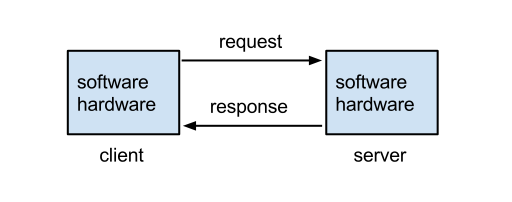
\includegraphics[width=1\textwidth]{figs/web.png}
    \legend{Fonte: https://commons.wikimedia.org/wiki/File:Client-server\_model.svg acessado dia 15 de dezembro de 2019 às 23:26}
    \label{fig:web}
\end{figure}

Uma aplicação web é um sistema projetado para ser executado em um navegador, essa é sua principal vantagem, visto que não será necessário alguns pré-requisitos como o uso de um sistema operacional em específico, por exemplo. Essa característica multiplataforma é ótima em relação a mobilidade e flexibilidade, pois em qualquer lugar/dispositivo que contém um navegador será possível acessar a aplicação. Além disso, as tecnologias para desenvolvimento web evoluíram muito, atualmente é possível fazer layouts que se adéquam fielmente aos \textit{smartphones}, buscando assim uma melhor experiência para o usuário\cite{pandey2013responsive}. \par
O sistema aqui proposto se encaixa muito bem em um modelo web, devido aos seus atores da aplicação necessitarem de portabilidade da aplicação, pois os mesmo se encontram em uma rotina corriqueira, devido ao deslocamento entre sua casa, estágio, universidade e afazeres em geral.

%\subsection{Guia do beneficiamento do cacau de qualidade}
%O guia \cite{guia_beneficiamento_cacau_2013}, fala da importância do beneficiamento das sementes de cacau e o passo a passo, com dicas e técnicas, para que o cacau seja produzido com elevado padrão de qualidade. 

%Em uma das seções, fala-se sobre como realizar a prova de corte, indicando como deve ser a escolha das amêndoas, a quantidade de porções e o peso de cada porção para que a seleção seja da forma mais aleatória possível, e então fala sobre a disposição das amêndoas para a análise visual, além de recomendar a análise olfativa e do paladar. 

%Possui algumas imagens indicando o passo a passo, as imagens de um exemplar de amêndoa de cada classe, e disponibiliza uma tabela de avaliação de qualidade, onde o produtor insere informações como a data da colheita, aroma, umidade e a classifica visualmente.

%O guia possui dados que auxiliam também a identificar a classe dado a tolerância máxima de percentuais de defeitos para amêndoas de cacau comercial, segundo a Instrução Normativa nº 38/2008 (MAPA).

%Guia do beneficiamento

%\subsubsection{\textit{Cocoa Beans Industry Quality Requirements}}
%A publicação \cite{cocoa_quality_requeriments_2016} é subdividido em três partes, onde a primeira fala sobre os aspectos de qualidade das sementes de cacau, a segunda que fala sobre os padrões de qualidade de cacau internacionais e outros padrões, e a terceira parte que aborda sobre como aspectos da produção do cacau afetam os requerimentos de qualidade.

%Na seção da prova de corte, dita as regras que devem ser seguidas para que haja a comprovação da qualidade das amêndoas, que são citadas em tópicos anteriores. É dito sobre o que é a prova de corte, qual a finalidade, a quantidade de amostras que deve ser selecionada, e sobre o corte a ser feito em cada amêndoa. Sobre as categorias classificadas pela ISO, e sobre o uso de apenas uma parte delas.

%Na mesma seção fala sobre outra forma de realizar o teste de qualidade, que é a contagem de sementes, onde é verificado a quantidade de sementes multiplicado por 100, e esse produto é dividido pela massa total dessas sementes selecionadas.

%
%\subsection{Cartilha de classificação CEPLAC}
%A cartilha \cite{cartilha_ceplac} informa sobre os passos do correto beneficiamento do cacau, desde sua colheita, a disposição em bananeiras, o descanso para consentração dos açucares, a quebra do cacau, o transporte para a casa de fermentação, o processo de fermentação e a secagem e são exibidos os defeitos das amêndoas.

%\subsection{Beneficiamento primário do cacau}

% Beneficiamento do cacau

%O folder \cite{folder_beneficiamento_ceplac} publicado pela CEPLAC do Pará fala sobre o passo a passo do beneficiamento, com figuras indicando ferramentas a passos do beneficiamento, e algumas tabelas com métricas para a construção de um cocho, e sobre os períodos de estiagem e chuva para que o cacau tenha uma boa fermentação.

%\subsection{Caracterização de amêndoas e chocolate de diferentes variedades de cacau visando a melhoria da qualidade tecnológica}

%O trabalho \cite{silva2013caracterizaccao} aborda sobre a qualidade do cacau, fatores que influenciam no sabor do chocolate, avaliação da qualidade do cacau, como a prova de corte e análise sensorial, o pré-processamento e processamento do cacau, que aborda desde a colheita e abertura dos frutos, até a moagem para obtenção do liquor e a prensagem para obtenção da torta e manteiga de cacau. Aborda também sobre o processamento do chocolate, tratando da mistura e refino, conchgem e temperagem, resfriamento e moldagem.

%A pesquisa trabalha sobre duas safras, atuando na caracterisação fisico-quimica, realizando análise descritiva e quantitativa, e o teste de aceitação dos chocolates.


%\subsection{Caracterização das sementes de variedades de cacau \textit{Theobroma cacao L.} resistentes à vassoura de bruxa durante a fermentação e após a secagem}

%O trabalho \cite{cruz2013caracterizaccao} possui como foco a caracterização das sementes de cacau resistentes à vassora de bruxa.

%No capítulo 1 apresenta o pré-processamento do cacau, que é abordado a colheita e quebra dos frutos, a fermentação, a secagem e o armazenamento. No tópico seguinte, aborda a avaliação da qualidade das amêndoas através da prova de corte. Aborda superficialmente a prova de corte.

%No capítulo 2 é abordado apenas o cacau proveniente de variedades resistentes à vassoura de bruxa.

\section{Linguagem Ruby}
Desenvolvida em 1995 por Yukihiro Matsumoto, Ruby é uma linguagem interpretada que inicialmente tinha objetivos muito semelhantes a linguagem Python\cite{purer2009phpvspythonvsruby}. Dinâmico e de código fonte aberto, a linguagem tem foco na simplicidade e produtividade, possui uma sintaxe elegante, natural e fácil de ler e escrever \cite{siteruby}. \par
Ruby segue o princípio de pouca surpresa, isso significa que a linguagem foi construída para ser intuitiva e com comportamentos esperados para o programador\cite{purer2009phpvspythonvsruby}. Diante disso, a curva de aprendizado da linguagem se torna muito baixa, encorajando assim outras pessoas a contribuir com o projeto desenvolvido aqui.

%\subsection{RGB}
%Amplamente conhecido, é um modelo de cor aditiva onde as cores vermelho, verde e azul são combinadas em diferentes intensidades produzindo outras cores. O RGB (vermelho, verde e azul) são chamadas de cores primárias.

%Na Figura \ref{fig:cor_RGB} podemos ver a representação do espaço de cor RGB.

%\begin{figure}[hbtp!]
% \centering
% \caption{Representação do espaço de cor RGB}
% \includegraphics[scale=0.07]{figs/RGB.png}
% \legend{Fonte: \cite{cor_RGB}}
% \label{fig:cor_RGB}
%\end{figure}

%\subsection{HSV}
%Hue (matiz): define o componente de cor, ou a posição no círculo.

%Saturation (saturação): define o quão "pura" é a cor, ou se ela está
%misturada com outras cores (complementar), tornando-a mais pálida.

%Value (valor/brilho): define a quantidade de luz na mistura, quanto
%mais luz mais clara a cor (na ausência de valor, a imagem é toda
%preta).

%Na Figura \ref{fig:cor_HSV} podemos ver a representação do espaço de cor HSV.

%\begin{figure}[hbtp!]
% \centering
% \caption{Representação do espaço de cor HSV}
% \includegraphics[scale=0.07]{figs/HSV.png}
% \legend{Fonte: \cite{cor_HSV}}
% \label{fig:cor_HSV}
%\end{figure}

\section{\textit{Framework}}
Em desenvolvimento de software, \textit{framework} é uma concepção de vários códigos comuns entre diversos projetos, buscando assim um kit de ferramentas genéricos para ser usado de acordo com a necessidade de cada projeto a ser implementado em cima dele. Segundo Fayad e Schmidt, framework é um conjunto de classes que colaboram para realizar uma responsabilidade para um domínio de um subsistema da aplicação\cite{frameworkwikipedia}. \par
As principais vantagens de \textit{frameworks} são: maior facilidade para debugar algum erro de implementação, foco na abstração de soluções do problema proposto, eficiência na resolução dos problemas e melhora no uso dos recursos\cite{frameworkwikipedia}. \par
O Ruby on Rails(RoR) teve sua primeira versão lançada em dezembro de 2005, foi desenvolvido pela 337Signal Inc com o objetivo de criar o projeto Basecamp, um gerenciamento colaborativo de projetos. Escrito em linguagem Ruby, RoR é um \textit{framework full-stack}(ou seja, possui ferramentas para desenvolvimento \textit{frontend} e \textit{backend}) para desenvolvimento de aplicativos web baseados em banco de dados\cite{plekhanova2009evaluating}. \par
Esse \textit{framework} foi escolhido para o projeto por alguns motivos, tanto pessoais como técnicos. Foi levado em consideração uma forte familiaridade da equipe executante com a linguagem de programação Ruby, devido aos mesmos utilizarem ela na vida acadêmica e profissional. Diante disso, a execução do projeto seria mais ágil e eficaz. Quando comparado com outros \textit{frameworks}, como Laravel, RoR é um dos mais utilizados, tem atualizações frequentes e uma vasta comunidade de código aberto, nitidamente terá um futuro seguro no mundo na programação \cite{verma2014mvc}. \par
Bootstrap é um \textit{framework web frontend} de código fonte aberto, baseando-se em modelo de design, teoria das cores, tipografia e Experiência do Usuário(UX – do inglês \textit{User Experience}) esse \textit{framework} serve para criar uma identidade visual forte e amigável para sistemas web, buscando melhorar o contato do usuário com o sistema\cite{bootstrapwikipedia}. Esse \textit{framework} conta atualmente com uma enorme popularidade que vem crescendo todos os dias \cite{jain2014review}. \par

%Na próxima seção é apresentado o OpenCV e alguns algoritmos que auxiliaram no processo de segmentação e que foram analisados neste trabalho.

%\newpage
%\subsection{Baseado em detecção de bordas}
%Primeiro aplica-se o método da morfologia matemática para detecção de bordas, que podem ser o de Sobel, Canny, Laplaciana, Prewit ou Roberts. Em seguida é feita um agrupamento de pixels detectados como bordas, a partir de um algoritmo de união ou realce de bordas, que permite determinar de maneira mais precisa o contorno dos objetos de uma imagem.
%Na Figura \ref{Border Detection} pode ser visto a utilização da técnica de detecção de bordas em manchas na pele.

%\begin{figure}[hbpt!]
% \centering
% \caption{Exemplo de segmentação utilizando detecção de bordas}
% \includegraphics[scale=0.3,angle=90]{figs/algoritmos/anisotropic_dermoscopy.png}
% \legend{Fonte: \cite{anisotropic_dermoscopy}}
% \label{Border Detection}
%\end{figure}

%\subsection{Baseado em regiões}
%Um conjunto de pixels que possuem determinado grau de similaridade, são tidos como regiões. No método de segmentação baseado em regiões, cada região é composta por pixels com um valor similar, baseado em um critério de similaridade. Na Figura \ref{Baseado em regiões} pode-se ver a técnica sendo aplicada na segmentação do milho e ervilha, ou de feijões de cores e tamanhos diferentes.

%\begin{figure}[hbpt!]
%\centering
%\caption{Exemplo de segmentação baseado em regiões}
%\begin{minipage}{.5\textwidth}
  %\centering
  %\includegraphics[width=.75\linewidth]{figs/opencv/region_growing_1.png}
%   \label{fig:test1}
%\end{minipage}%
%\begin{minipage}{.5\textwidth}
  %\centering
  %\includegraphics[width=.75\linewidth]{figs/opencv/region_growing_2.pn%g}
%   \label{fig:test2}
%\end{minipage}
%\legend{Fonte: \cite{region_growing}}
%\label{Baseado em regiões}
%\end{figure}


%\subsection{Transformação divisória (Watershed)}

%São algoritmos que possuem como base a morfologia matemática, que permite extrair as bordas existentes em uma imagem, e é também uma técnica de segmentação baseada em regiões. Imagina-se os valores dos pixels da imagem como um gráfico topográfico 3D, onde o 'x' e 'y' são coordenadas do plano e 'z' são os valores dos pixels. O objetivo principal é encontrar as linhas divisórias em uma imagem para separar diferentes regiões, que correspondem aos mínimos do gradiente morfológico. Na Figura \ref{Watershed} pode ser visto a utilização da técnica do watershed para segmentação de uma imagem.

%\begin{figure}[hbpt!]
% \centering
% \caption{Exemplo de segmentação utilizando watershed}
% \includegraphics[scale=0.4]{figs/algoritmos/elephant.jpg}
% \legend{Fonte: \cite{watershed_citation}}
% \label{Watershed}
%\end{figure}

\section{Banco de dados}
\label{sec:opencv}

Segundo \cite{ceri2013logic}, “sistemas de banco de dados lidam com grandes coleções de dados compartilhados e com memória de massa e fornecem a tecnologia para suportar recuperação eficiente e atualização confiável de dados persistentes”. \par
O banco de dados baseado no modelo relacional foi arquitetado há mais de 35 anos com o objetivo de atender ao processamento de dados, desde então, tornou-se a melhor opção para armazenar informações. O modelo Não Relacional(NoSQL) é baseado em arquivos e foi desenvolvido por Carlo Strozzi em 1998, modelo ao qual omite o uso da linguagem SQL.\cite{mohamed2014relationalvsnosql} \par
No projeto em questão será utilizado o modelo relacional, pois o NoSQL ainda não atingiu uma maturidade completa devido ao seu surgimento recente, outro ponto é a escassez em segurança dos bancos NoSQL como demonstrado na tabela 1\cite{mohamed2014relationalvsnosql}: \par

\begin{table}[ht]
\centering
\caption{Tabela de comparação entre banco de dados relacionais e não relacionais}
\label{tab:sqlvsnosql}
\begin{flushright}
\footnotesize
(continua)
\end{flushright}
\resizebox{\textwidth}{!}{%
\begin{tabularx}{0.9\textwidth} { 
  | >{\raggedright\arraybackslash}X 
  | >{\raggedright\arraybackslash}X 
  | >{\raggedright\arraybackslash}X | }
 \hline
 Categoria & Modelo relacional & Modelo não-relacional \\
 \hline
 Autenticação  & Todos os bancos de dados relacionais vieram com mecanismo de autenticação e podem escolher qualquer um desses mecanismos a serem usados.  & Muitos bancos de dados NoSQL, por padrão, não vêm com mecanismo de autenticação ou autorização, mas podem usar algum método externo para executar esta operação.  \\
\hline
Integridade dos dados & As propriedades ACID(acrônimo de Atomicidade, Consistência, Isolamento e Durabilidade) usadas nos bancos de dados relacionais garantem que as transações do banco de dados sejam processadas com confiabilidade, garantindo a integração dos dados. & Eventualmente consistente é um dos princípios das propriedades BASE, portanto, a integridade dos dados nem sempre é alcançada nos bancos de dados NoSQL. \\
\end{tabularx}%
}
\end{table}
\pagebreak

\begin{table}[ht]
\centering
Tabela \ref{tab:sqlvsnosql} – Tabela de comparação entre banco de dados relacionais e não relacionais
\begin{flushright}
\footnotesize
(conclusão)
\end{flushright}
\resizebox{\textwidth}{!}{%
\begin{tabularx}{0.9\textwidth} { 
  | >{\raggedright\arraybackslash}X 
  | >{\raggedright\arraybackslash}X 
  | >{\raggedright\arraybackslash}X | }
 \hline
 Categoria & Modelo relacional & Modelo não-relacional \\
\hline
Confidencialidade & A confidencialidade dos dados geralmente é alcançada no banco de dados relacional porque foi usada técnicas de criptografia para armazenar dados criptografados. & A confidencialidade dos dados não é alcançada, porque geralmente os dados são armazenados de forma clara. \\
\hline
Auditoria & Fornecer mecanismos auditar que permita escrever para o arquivos syslog ou xml do banco de dados, e alguns dar uma auditoria mais avançada. & A maioria do NoSQL bancos de dados não fornecer auditoria. Existem alguns bancos de dados que fornecem auditoria com questões como Couchdb que loja o nome de usuário e senha no log arquivo que é claro compromete a segurança. \\
\hline
Comunicação com o cliente & Os bancos de dados relacionais oferecem mecanismo seguro de comunicação com o cliente usando protocolos de criptografia e \textit{Secure Sockets Layer}(SSL). & A maioria dos bancos de dados NoSQL não oferecem mecanismos de comunicação segura com o cliente. \\
\hline
\end{tabularx}%
}
\end{table}

%OpenCV-Python é uma API Python para OpenCV, combinando as melhores qualidades da API OpenCV para C++ e a linguagem Python \cite{opencv_python_api}.

%A biblioteca OpenCV-Python é destinada a resolução de problemas de visão computacional, ela faz uso do Numpy, que é uma biblioteca altamente otimizada para operações numéricas que utiliza o estilo de sintaxe do MATLAB. Todas as estruturas de array do OpenCV são convertidas para e de arrays Numpy. Isso permite facilitar a integração com outras bibliotecas que utilizam Numpy como a SciPy e Matplotlib \cite{opencv_python_api}.

%O threshold se baseia na diferença de tons de cinza que compõem diferentes objetos na imagem. A partir das características dos objetos que se quer isolar (obtidos por meio de um histograma por exemplo), a imagem será segmentada em dois grupos: os que possuem níveis de cinza abaixo do valor estabelecido, e os que possuem níveis de cinza acima do valor estabelecido. Para a geração de uma imagem limiarizada, atribui-se um valor fixo para todos os pixels de um mesmo grupo. A imagem gerada será binária, ou seja,  terá  apenas  dois valores  possíveis  para  cada  pixel. Na Figura \ref{Thresholding} podemos ver um exemplo de utilização de thresholding em olhos.

%\begin{figure}[hbpt!]
% \centering
% \caption{Exemplo de utilização do thresholding}
% \includegraphics[angle=270,scale=0.4]{figs/algoritmos/pathologies_thresholding.png}
% \legend{Fonte: \cite{pathologies_thresholding}}
% \label{Thresholding}
%\end{figure}

\section{Engenharia de software}

Engenharia de software é uma área da computação voltada à especificação, desenvolvimento, manutenção e criação de software, com a  aplicação de tecnologias e práticas de gerência de projetos e outras disciplinas, visando organização, produtividade e qualidade\cite{engenhariawikipedia}. Por um lado engenharia de software possui características explícitas de produção e engenharia devido ao processo de criação do produto(software). Por outro lado é exigido uma melhoria contínua e sequencial da qualidade do produto e do processo de criação do software, nesse contexto é enxergado como ciência\cite{travassos2002introducao}.

%O OpenCV conta com mais de 150 métodos de conversão do espaço de cores, mas o BGR <-> Cinza e BGR <-> HSV são os mais utilizados. A função tem o escopo Imgproc.cvtColor(imagem\_entrada, imagem\_saida, flag) onde \textit{flag} determina o tipo de conversão.

%Para RGB -> Cinza utiliza-se a \textit{flag} Imgproc.COLOR\_BGR2GRAY e para RGB -> HSV utiliza-se a \textit{flag} cv2.COLOR\_BGR2HSV. Um exemplo de conversão de escala de cor de RGB (Figura \ref{fig:lenna_rgb}) para Cinza (Figura \ref{fig:lenna_gray}) pode ser visualizado na Figura \ref{fig:rgb2gray}.

\subsection{Padrão de Projeto MVC (Model View Controller)}
\label{subsec:thresholding}

O padrão \textit{model-view-controller}(MVC) é um padrão de projeto(do inglês \textit{design pattern}) de apresentação/abstração/controle utilizado para arquitetar sistemas de softwares \cite{leff2001webmvc}. No paradigma MVC separa a aplicação em três tipos de objetos, cada um especializado em sua tarefa, são elas: Modelo(\textit{Model}), Visão(\textit{View}) e Controlador(\textit{Controller}). \par
O \textit{Model} gerencia e valida o comportamento dos dados da aplicação, conversando com o banco de dados, por exemplo. A \textit{View} é a parte gráfica da aplicação ao qual irá interagir visualmente com o usuário. O \textit{Controller} interpreta, ordena e responde a requisições feitas pelos usuários.\cite{burbeck1997applications} A figura \ref{fig:mvc} exemplifica muito bem a abordagem do MVC. \par

\begin{figure}[htbp!]
  \centering
  \caption{Fluxo do padrão MVC}
  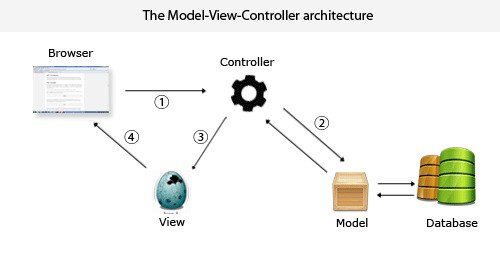
\includegraphics[width=1\textwidth]{figs/mvc.jpg}
    \legend{Fonte: https://www.cuelogic.com/blog/hello-world-in-ruby-on-rails-and-folder-structure acessado dia 16 de dezembro de 2019 às 08:15}
    \label{fig:mvc}
\end{figure}

%As transformações morfológicas são operações simples baseadas na forma da imagem. Normalmente utilizado em imagens binárias. A função necessita de dois parâmetros, um é a imagem de entrada, o outro é o elemento estruturante, ou kernel, que decide a natureza da operação. Duas operações morfológicas básicas são a erosão e a dilatação.

%A ideia básica da erosão é servir como uma erosão do solo, removendo ruídos ou reduzindo bordas do objeto. A dilatação é a ideia oposta da erosão, cujo objetivo é aumentar as bordas do objeto. Normalmente, em caso de remoção de ruídos, a erosão é sucedida de dilatação.

\subsection{Testes automatizados}

Segundo \cite{mathur1991performance}, “A confiabilidade do software é uma medida do desempenho de um programa em seu ambiente operacional”. Para elevar a confiabilidade é necessário recorrer a métodos de testes. Existem vários tipos de testes de softwares, e cada um se aplica em um estágio do desenvolvimento do software, pois cada um tem objetivos diferentes\cite{nidhra2012black}. \par
No projeto proposto será implementado tais testes: \par
\begin{itemize}  
\item Testes unitários, aos quais testa um componente isolado ou classe do sistema;
\item Testes de integração, aos quais combinam vários componentes do software para testar se funcionam de maneira satisfatória;
\item Teste de segurança, responsável por testar se os dados são acessados de maneira segura;
% \item Teste funcional, encarregado de testar se os requisitos funcionais foram alcançados.
\end{itemize}
Testes funcionais, de sistema, de aceitação e beta não foram incluídos devido a sua característica de necessitar pessoas independentes ao projeto para testar o software.

\section{Projetos de código fonte aberto}
OSS(\textit{Open Source Software}) é um termo usado para designar um software desenvolvido e lançado sob algum tipo de licença de código aberto. Atualmente existem várias licenças com uma gama de características diferentes, mas todas necessitam da permissão do código fonte do software\cite{crowston2003defining}.

Algumas vantagens de projetar um OSS são:
\begin{itemize}  
\item oferta gratuita de código aumentará a participação de mercado\cite{fitzgerald2006transformation}
\item construir uma base de desenvolvimento em torno da ferramenta aumentar a sustentabilidade a longo prazo\cite{nyman2011forking}
\item O conjunto crescente de partes interessadas resulta em melhorias adicionais sucessivas no software\cite{heron2013open}
\item Replicação dos resultados obtidos neste projeto
\end{itemize}


\section{Trabalhos correlatos}
\label{sec:java}

Foram pesquisados alguns trabalhos, porém nenhum se encaixou perfeitamente com os objetivos do projeto aqui desenvolvido. Entretanto, alguns projetos têm cunho semelhante. \par
O sistema Ifood é usado para delivery de comida, buscando conectar vendedores com clientes. Disponível para plataformas Android, IOS e web o sistema recebe mais de 6,2 milhões de pedidos mensais\cite{bastos2018marketing}. Após efetuar seu login, o cliente pode realizar seu pedido informando a localização onde deseja que a entrega seja feita. A forma de pagamento pode ser feita pelo próprio sistema. A figura \ref{fig:ifood} apresenta o fluxo básico para realizar e acompanhar pedidos realizados pelo aplicativo.

\pagebreak
\begin{figure}[htbp!]
  \centering
  \caption{Fluxo de uso do aplicativo ifood}
  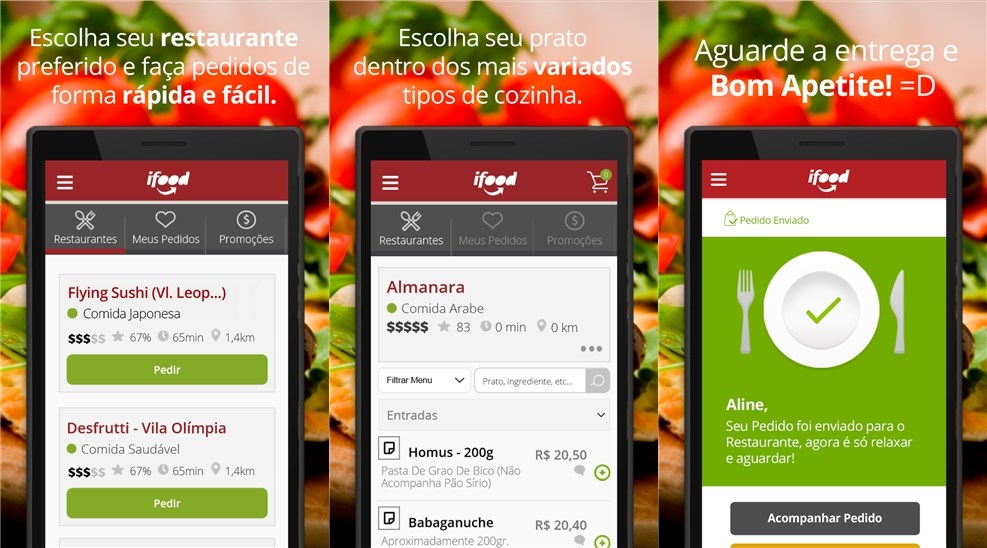
\includegraphics[width=1\textwidth]{figs/ifood2.jpg}
    \legend{Fonte: https://cadernomercado.com.br/pesquisa-do-ifood-revela-habitos-de-consumo-no-delivery/ acessado dia 15 de dezembro de 2019 às 23:26}
    \label{fig:ifood}
\end{figure}
\chapter{Desenvolvimento do sistema}
\label{chap:etapas_desenvolvimento}

Nesta seção iremos apresentar detalhadamente os passos e ferramentas necessárias para elaboração da aplicação web Mercado Universitário. A medida que for sendo detalhado cada passo seguido, será apresentada sua finalidade e o motivo do uso das ferramentas ali utilizadas para produção do mesmo. \par
Intencionalmente as seções estão organizadas de forma cronológica a linha de desenvolvimento da aplicação, dessa forma fica mais fácil o entendimento e execução futura dos passos necessários para validar o atual projeto por terceiros. Foi buscado não só organizar as subseções desta seção, bem como seguir uma metodologia ágil de desenvolvimento para construção do sistema web, como será apresentado na próxima subseção.

\section{Método ágil de desenvolvimento}

Desenvolvimento Guiado a Testes(TDD - do inglês Test Driven Development) foi a metodologia ágil de desenvolvimento para produção dessa aplicação devido a vários fatores, como:
\begin{itemize}  
\item Necessidade de \textit{feedbacks} rápidos sobre as funcionalidades implementadas sistema
\item Como o código será aberto, fica mais fácil a verificação de códigos bons e sem \textit{bugs} feitos por terceiros
\item A produtividade aumenta bastante, devido a ser fácil a detecção de \textit{bugs} por meio dos testes do TDD
\item Como será um projeto que estará constantemente sendo atualizado, fica-se mais fácil a implementação de novas funcionalidades e \textit{refactoring} do observando se tal mudança afeta outras partes do sistema.
\end{itemize}

\subsection{Bibliotecas utilizadas}
O RoR conta vantagem com toda a estrutura das RubyGems da linguagem de programação Ruby, que é um gerenciador de pacotes que fornece um padrão de formato para distribuição de bibliotecas, chamadas de \textit{gem}. Várias \textit{gems} foram utilizadas no atual projeto, muitas delas para facilitar o desenvolvimento, como outras que busca melhorias no código. A seguir será apresentado algumas delas:
\subsubsection{RSpec}\label{rspec}
RSpec é um \textit{framework behaviour-Driven Development}(BDD) de código aberto disponível no Github\footnote{Gem RSpec \url{https://github.com/rspec/rspec}} escrito em Ruby, que permite e facilita a automatização de testes no projeto. Com o RSpec é possível implementar vários tipos de testes, são eles: testes de \textit{model}, testes de \textit{controller} e testes de \textit{view}.
\subsubsection{Rubocop}\label{rubocop}
Rubocop é uma \textit{gem} de código fonte aberto disponível no Github\footnote{Gem Rubocop \url{https://github.com/rubocop-hq/rubocop}} que percorre e verifica se o código segue as boas práticas de programação definidas pelo guia de estilo Ruby. Tal \textit{gem} ajuda a manter os padrões sem que seja preciso conhecer literalmente todas as definições.
\subsubsection{Brakeman}\label{brakeman}
O Brakeman é uma \textit{gem} de código livre disponível no Github \footnote{Gem Brakeman \url{https://github.com/presidentbeef/brakeman}} que ajuda a descobrir várias vulnerabilidades de segurança do projeto. O brakeman roda de forma totalmente automatizada, buscando falhas como \textit{SQL Injection, File Access, Mass Assignment}, dentre outros. Então para ter uma aplicação segura e de qualidade é indispensável o uso dessa \textit{gem}.

No projeto Mercado Universitário foi aplicado três tipos de testes automatizados fornecidos pelo TDD, os testes unitários, os testes de integração e testes de segurança da aplicação. Tais testes serão melhor detalhados na seção \ref{tdd}.

\section{Atores do sistema}

Para que seja possível definir melhor o escopo dos requisitos do sistema(que será apresentado na seção \ref{requisitos}), foi preciso identificar os atores que farão parte da aplicação. Dessa forma será possível determinar e entender de maneira correta as responsabilidades de cada tipo de usuário do sistema. \par
Cada ator terá seu nível de acesso definido na aplicação, que será percebido na coluna “responsabilidade” que se encontra no quadro 1. Como pode ser percebido no quadro 1, os tipos de atores podem realizar tarefas distintas como também tarefas que têm um mesmo propósito. \par
Em tal projeto, inicialmente, não será necessário a presença de um ator como administrador geral do sistema devido a se tratar de um projeto piloto em uma única universidade, sem a necessidade constante de adicionar novas universidades e cursos da mesma. Tal ponto será apresentado e discutido melhor na seção de trabalhos futuros que se encontra na seção \ref{chap:conclusoes_trabalhos_futuros}.

\begin{table}[ht]
\centering
\caption{Tabela de atores do sistema}
\label{tab:atores}
\resizebox{\textwidth}{!}{%
\begin{tabularx}{0.9\textwidth} { 
  | >{\raggedright\arraybackslash}X 
  | >{\raggedright\arraybackslash}X 
  | >{\raggedright\arraybackslash}X 
  | >{\raggedright\arraybackslash}X | }
 \hline
 Ator & Descrição & Responsabilidade & Acesso a área restrita? \\
 \hline
 Convidado  & Qualquer pessoa do âmbito universitário que deseja comprar ou vender produtos  & Cadastrar-se como novo usuário do sistema & Não  \\
\hline
Cliente & Discentes, funcionários, ou moradores da região próxima a universidade & Visualizar categorias, produtos, vendedores, \textit{reviews} e seus próprios pedidos; Cadastrar novos pedidos e \textit{reviews}; Atualizar seus próprios \textit{reviews} e dados cadastrais & Não \\
\hline
Vendedor & Discentes, funcionários, ou moradores da região próxima a universidade que obtém renda a partir do comércio informal & Visualizar clientes, seus pedidos e seus \textit{reviews}; Cadastrar novos produtos; Atualizar seus produtos e dados cadastrais & Sim \\
\hline
\end{tabularx}%
}
\end{table}

\section{Levantamento de requisitos}\label{requisitos}

O levantamento de requisitos é completamente fundamental para a elaboração do desenvolvimento desse sistema, pois é nessa fase que entende-se o problema e as necessidades dos \textit{stakeholders}(Grupo de interesses) para propor as melhores soluções possíveis para resolução desse problema. Nesta seção iremos apresentar os requisitos funcionais e não funcionais do sistema.

\subsection{Requisitos funcionais}

Tais requisitos são necessários para atender as regras de negócio do sistema web, como o próprio nome já diz, são as funcionalidades do sistema.  Segundo \cite{sommerville2007engenharia}, os requisitos funcionais são as asserções de serviços que a aplicação deve proporcionar, como o sistema deve responder a entradas específicas e como o sistema deve proceder em determinadas situações. \par
Será definidas as seguintes denominações de prioridade de implementação no sistema:
\begin{itemize}  
\item \textbf{Essencial:} requisito imprescindível para o funcionamento do sistema em que o sistema. Em sua ausência, o sistema não entra no ar.
\item \textbf{Importante:} requisito em que deve ser implantado o mais rápido possível, pois sem o qual o sistema entra em funcionamento, mas de forma não satisfatória.
\item \textbf{Desejável:} requisito ao qual pode ser implantado sem pressa, pois não compromete o funcionamento do sistema, já que o mesmo funciona de forma satisfatória sem ele.
\end{itemize} \par
Não será necessário abordar todos os requisitos funcionais nesta seção, pois muitas vezes trata-se de requisitos parecidos e muitas vezes facilmente dedutíveis. Diante disso, serão apresentados apenas os principais para que tenha-se uma visão geral deles. A lista contendo todos os requisitos funcionais estará nos apêndices.

\textbf{RF02 - Fazer login} \par
\textbf{Prioridade:} Essencial \par
\textbf{Atores:} Cliente \par
\textbf{Descrição:} Após realizar o cadastro, o usuário estará apto a fazer o login na plataforma para ter acesso a todo o ambiente que o sistema proporciona. O login é totalmente essencial por ter a capacidade de identificar unicamente cada usuário do sistema por meio do seu e-mail e senha, fazendo assim com que o resto do sistema traga informações relativas em relação aquele ator que acabou de logar, como por exemplo retornar apenas compras realizadas pelo ator logado. \par
\textbf{Fluxo de eventos:} \par
\textbf{Principal} \par
\begin{enumerate}
  \item O usuário insere suas credenciais(e-mail e senha) e clica no botão para logar
  \item O sistema redireciona para a página de produtos e informa que o login foi bem sucedido.
\end{enumerate}

\textbf{Secundário}

\begin{enumerate}
  \item O usuário insere suas credenciais(e-mail e senha) e clica no botão para logar
  
  \item O sistema renderiza a mesma página e informa que o login não foi bem sucedido devido a divergência nos dados cadastrais
  
  \item O usuário corrige as credenciais no formulário e realiza uma nova submissão dos dados

\end{enumerate}

\textbf{RF08 - Cadastrar \textit{review} de um vendedor} \par
\textbf{Prioridade:} Essencial \par
\textbf{Atores:} Cliente \par
\textbf{Descrição:} O cliente poderá compartilhar sua opinião acerca de algum vendedor por meio da página de cadastro de \textit{review}, colocando em um formulário a descrição e nota(entre 1 e 5, inclusos) do vendedor. \par
\textbf{Fluxo de eventos:} \par
\textbf{Principal} \par
\begin{enumerate}
  \item O cliente acessa a página específica do vendedor
  \item Clica no link “deixe sua opinião!”
  \item Será redirecionado para página de cadastro de \textit{review}
  \item Preenche o formulário
  \item Submete os dados
  \item Será redirecionado para página do vendedor informando que a operação foi bem sucedida
\end{enumerate}

\textbf{RF10 - Adicionar produto ao carrinho de compras} \par
\textbf{Prioridade:} Essencial \par
\textbf{Atores:} Cliente \par
\textbf{Descrição:} Para compor um pedido, é necessário adicionar produtos ao pedido. O cliente poderá fazer isso diretamente na página do produto em que deseja comprar, colocando assim a quantidade desejada e clicando em “adicionar produto”. \par
\textbf{Fluxo de eventos:} \par
\textbf{Principal} \par
\begin{enumerate}
  \item Na página do produto, o cliente insere a quantidade do produto para ser adicionado
  \item Clica em “adicionar produto“
  \item Será redirecionado para página de produto com a notificação informando que a operação foi bem sucedida
\end{enumerate}

\textbf{RF11 - Visualizar pedidos} \par
\textbf{Prioridade:} Essencial \par
\textbf{Atores:} Cliente e vendedor \par
\textbf{Descrição:} Por meio do link “meus pedidos” na navbar será possível visualizar a lista de pedidos feitos(já realizados e que estão a realizar) pelo cliente. O vendedor conseguirá acessar a página pelo mesmo link do cliente, entretanto será mostrado apenas os pedidos já recebidos pelo vendedor, independentemente do status da compra ao qual o pedido se encontra. \par
\textbf{Fluxo de eventos:} \par
\textbf{Principal} \par
\begin{enumerate}
  \item O cliente acessa a página de pedidos pelo link do navbar
  \item Será renderizado duas sessões de lista de pedidos: pedidos já realizados e pedidos em aberto
  \item O cliente terá a opção de realizar os pedidos em aberto
\end{enumerate}

\textbf{RF12 - Cadastrar conta de vendedor} \par
\textbf{Prioridade:} Essencial \par
\textbf{Atores:} Cliente \par
\textbf{Descrição:} Para se tornar um vendedor, necessariamente é preciso que o ator seja um cliente, para então realizar o devido cadastro da conta. Só será possível uma conta de vendedor para cada conta cliente. O link denominado “seja um vendedor” para cadastro da conta estará disponível no navbar da aplicação. \par
\textbf{Fluxo de eventos:} \par
\textbf{Principal} \par
\begin{enumerate}
  \item O cliente clica no link “seja um vendedor” no navbar
  \item Será redirecionado para a página com um formulário para inserir os dados do vendedor
  \item Preenche os campos
  \item Submete os dados para ser cadastrado no banco de dados
  \item É redirecionado para a área restrita sendo informado que o cadastro foi realizado com sucesso
\end{enumerate}

\textbf{RF16 - Realizar pedido de compra} \par
\textbf{Prioridade:} Essencial \par
\textbf{Atores:} Cliente \par
\textbf{Descrição:} O ato de realizar o pedido é um recurso fundamental para a aplicação. Este requisito efetua a conexão entre um cliente e o vendedor(que no caso seria o fornecedor dos produtos do pedido em questão). Nessa etapa será possível deixar um recado para o vendedor e selecionar o local de entrega(caso o vendedor realize entregas). \par
\textbf{Fluxo de eventos:} \par
\textbf{Principal} \par
\begin{enumerate}
  \item O cliente clicará no link “meus pedidos” no navbar
  \item Será redirecionado para a página com a lista de pedidos fechados e abertos
  \item Preencherá um recado para o vendedor
  \item Escolherá o tipo de entrega/local do pedido
  \item Realiza o pedido clicando no botão “realizar pedido”
  \item Será renderizada a mesma página informando que o pedido foi efetivado
\end{enumerate}

\textbf{RF21 - Línguas estrangeiras} \par
\textbf{Prioridade:} Desejável \par
\textbf{Atores:} Cliente e Vendedor \par
\textbf{Descrição:} Por ter um nicho universitário, muitas das vezes pessoas de outros países tem contato com esse âmbito, pessoas essas que podem não falar o idioma português. Dessa forma, é desejável que o sistema seja bilíngue, suportando o idioma nativo(português) e um idioma bastante difundido(inglês). A mudança de idioma ocorrerá a qualquer momento de uso do sistema, bastando um clique para que os textos estáticos da aplicação alterne entre tais idiomas. \par
\textbf{Fluxo de eventos:} \par
\textbf{Principal} \par
\begin{enumerate}
  \item O usuário acessa a aplicação
  \item Clica na bandeira referente ao idioma desejado
  \item A página é renderizada com o novo idioma
\end{enumerate}

\subsection{Requisitos não funcionais}
De acordo com \cite{sommerville2007engenharia}, os requisitos não funcionais são requisitos que não estão diretamente relacionados com serviços específicos oferecidos pelo sistema a seus usuários. Eles estão associados às características emergentes do sistema, como confiabilidade, tempo de resposta e ocupação de área. Na tabela 1 será apresentado os requisitos não funcionais atribuídos ao sistema.

\begin{table}[ht]
\centering
\caption{Tabela de requisitos não funcionais do sistema}
\label{tab:naofuncionais}
\begin{flushright}
\footnotesize
(continua)
\end{flushright}
\resizebox{\textwidth}{!}{%
\begin{tabularx}{0.9\textwidth} { 
  | >{\raggedright\arraybackslash}X 
  | >{\raggedright\arraybackslash}X 
  | >{\raggedright\arraybackslash}X | }
 \hline
 Referência & Descrição & Atributo \\
 \hline
 RNF01 & O sistema deve ser desenvolvido utilizando a linguagem de programação Ruby na versão 2.6+. & Implementação  \\
 \hline
 RNF02 & A versão do \textit{framework} RoR deve ser 5.2+. & Implementação  \\
 \hline
 RNF03 & O sistema deve utilizar o Sistema Gerenciador de Banco de Dados(SGBD) MariaDB na versão 10.4+. & Implementação  \\
 \hline
 RNF04 & Deverá aparecer mensagens de sucesso, informativas e erro abaixo do navbar da aplicação utilizando cores condizentes com o tipo da mensagem. & Usabilidade  \\
 \hline
 RNF05 & O sistema deverá rodar em qualquer plataforma. & Implementação  \\
 \hline
 RNF06 & O sistema deverá ter alta disponibilidade, funcionando 24 horas por dia. & Confiabilidade  \\
\end{tabularx}%
}
\end{table}

\begin{table}[ht]
\centering
Tabela \ref{tab:naofuncionais} – Tabela de requisitos não funcionais do sistema
\begin{flushright}
\footnotesize
(conclusão)
\end{flushright}
\resizebox{\textwidth}{!}{%
\begin{tabularx}{0.9\textwidth} { 
  | >{\raggedright\arraybackslash}X 
  | >{\raggedright\arraybackslash}X 
  | >{\raggedright\arraybackslash}X | }
 \hline
 Referência & Descrição & Atributo \\
 \hline
 RNF07 & A aplicação deve possuir segurança em operações por nível de usuário. & Segurança  \\
 \hline
\end{tabularx}%
}
\end{table}


%  \hline
%  RNF07 & A aplicação deve possuir segurança em operações por nível de usuário. & Segurança  \\

\section{Engenharia de software}
Nesta subseção será apresentado vários diagramas baseados em engenharia de software para ajudar a entender, agilizar e organizar todo o escopo da aplicação a ser desenvolvida.

\subsection{Modelo de entidade e relacionamento}
Para criar um sistema bem estruturado, é de suma importância que seja feito o diagrama de entidade e relacionamento do banco de dados da aplicação. Nele estará disposto todas as tabelas da aplicação, facilitando assim o desenvolvimento do sistema, isso traz consigo grande produtividade, uma vez que não será necessário grandes mudanças na estrutura a cada passo de elaboração da aplicação.

A figura \ref{fig:err}, expõe o modelo de entidade e relacionamento atual do sistema, modelo esse que passou por diversas mudanças básicas ao decorrer do desenvolvimento, como inserção e exclusão de atributos das tabelas. Essas alterações no banco são facilitadas por meio das \textit{migrations}, que são técnicas e ferramentas que auxiliam o versionamento do banco de dados durante o desenvolvimento da aplicação.

\begin{figure}[htbp!]
  \centering
  \caption{Diagrama de entidade e relacionamento do banco de dados}
  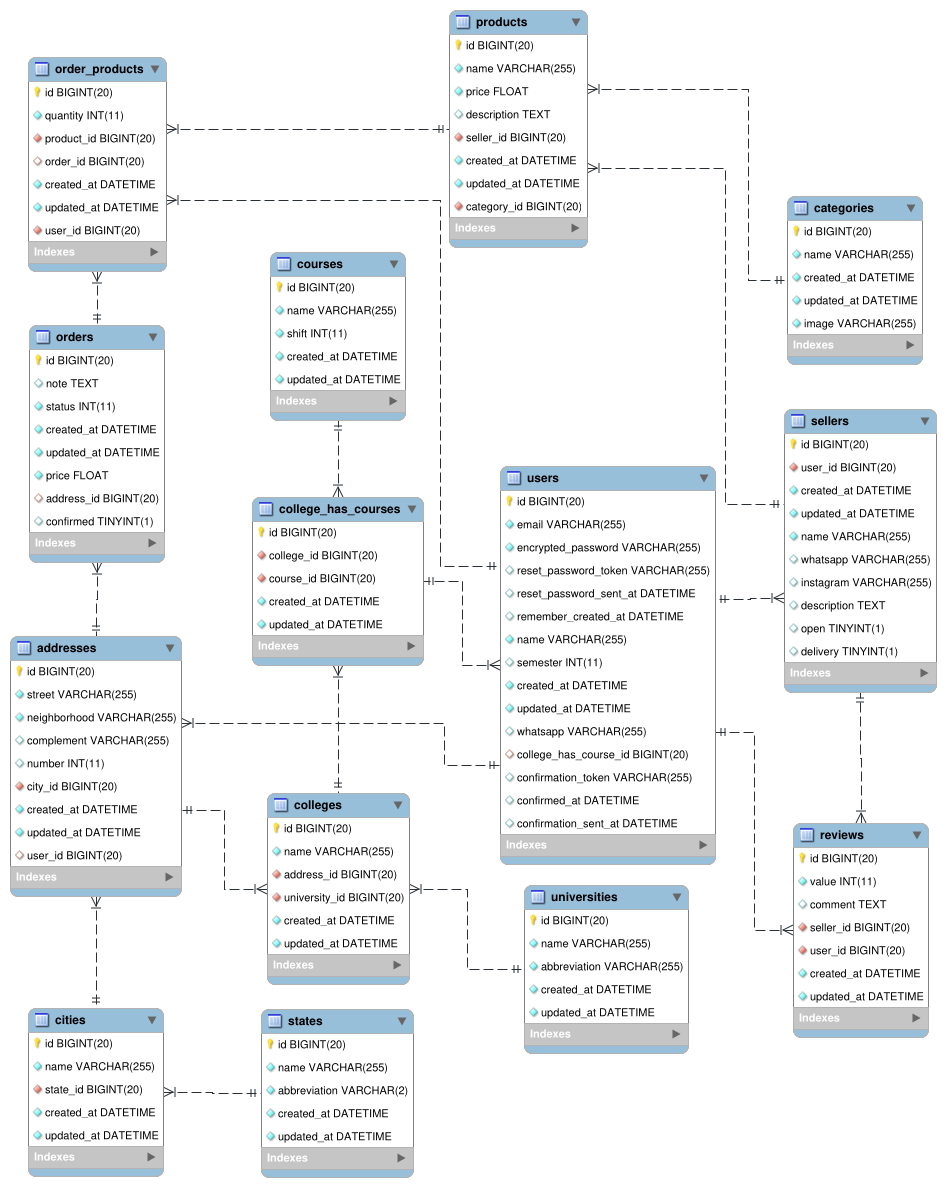
\includegraphics[width=1\textwidth]{figs/err.png}
    \legend{Fonte: Elaborada pelo autor.}
    \label{fig:err}
\end{figure}

\subsection{Telas de \textit{mockup}}\label{mockup}
Foi necessário prototipar a aplicação antes do desenvolvimento, pois com essa abordagem ficou mais fácil e objetivo o desenvolvimento do sistema. Para confecção de cada tela de \textit{mockup}, foi-se utilizada a ferramenta Figma.

O Figma é uma ferramenta de design de interface. Um dos motivos para usar essa ferramenta no projeto foi devido a mesma possuir uma portabilidade muito boa, visto que roda diretamente no navegador, ou seja, é compatível com Windows, Linux e Mac. É multitarefas, ou seja, uma equipe pode explorar o mesmo projeto juntas e ver as alterações em tempo real.

A elaboração dessa etapa foi de suma importância para o resultado final do projeto. Então, para um melhor aproveitamento do dados produzidos, na seção \ref{chap:resultados} será realizada uma comparação entre as telas de \textit{mockup} e o resultado final da aplicação.

\subsection{Diagrama de casos de uso}
O diagrama de casos de uso é de grande importância para um entendimento geral do sistema, apresentando as principais ações que cada usuário pode fazer. Esse diagrama é apresentado na figura \ref{fig:use}. O cliente pode realizar basicamente três ações. Já pelo vendedor é capaz de realizar outras duas ações além das permitidas quando o mesmo se encontra no papel de cliente do sistema. Em todos os casos é necessário que seja realizado o login na aplicação.
\begin{figure}[htbp!]
  \centering
  \caption{Diagrama de caso de uso}
  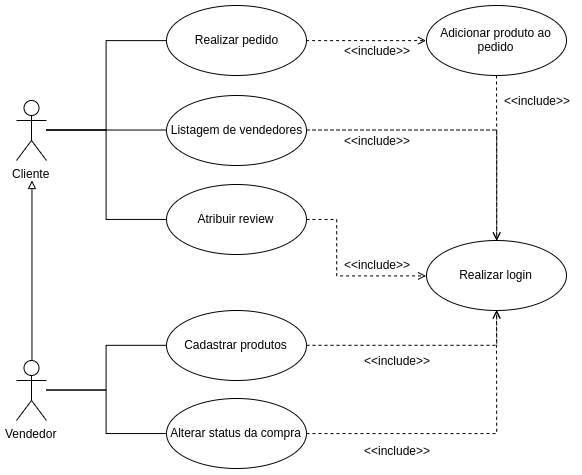
\includegraphics[width=1\textwidth]{figs/caso_de_uso.png}
    \legend{Fonte: Elaborada pelo autor.}
    \label{fig:use}
\end{figure}


\subsection{Diagrama de sequência}
Por meio dos diagramas de sequência será possível ter uma boa visão em relação a cada passo para concluir determinada ação. Nessa seção será apresentado alguns diagramas de sequência que cobrem a todas as funcionalidades do sistema.

\subsubsection{Cadastrar um produto}
Para cadastrar um produto no sistema, será necessário que o usuário tenha perfil tanto de cliente como de vendedor e esteja logado no sistema. Com isso, será possível acessar a área restrita do sistema e solicitar um novo cadastro de produto, inserido cada campo e submetendo para que o registro seja efetuado no banco de dados. Tal diagrama pode ser observado na figura \ref{fig:sequence1}.
\begin{figure}[htbp!]
  \centering
  \caption{Cadastrar um produto}
  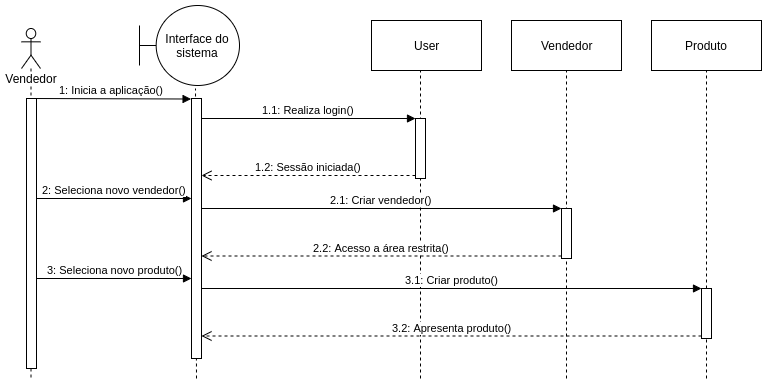
\includegraphics[width=1\textwidth]{figs/sequence1.png}
    \legend{Fonte: Elaborada pelo autor.}
    \label{fig:sequence1}
\end{figure}

\subsubsection{Atribuir um review}
A atribuição de um \textit{review} é uma ação simples, ao qual será necessário que o usuário acesse a página individual do vendedor e clique no link ser redirecionado para a página de inserção do \textit{review}, bastando definir a nota e comentário e submeter ao sistema. Tal diagrama pode ser observado na figura \ref{fig:sequence2}.
\begin{figure}[htbp!]
  \centering
  \caption{Atribuir um review}
  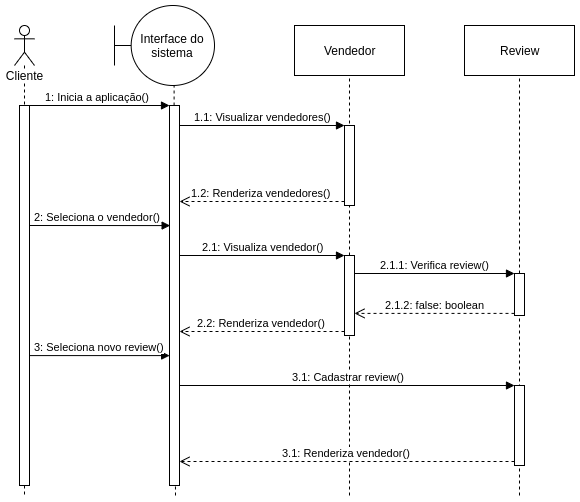
\includegraphics[width=1\textwidth]{figs/sequence2.png}
    \legend{Fonte: Elaborada pelo autor.}
    \label{fig:sequence2}
\end{figure}

\subsubsection{Realizar um pedido}
% escrever aqui
A ação de realizar um pedido é a principal do sistema, ao qual será realizada por um cliente. Será necessário que o cliente insira no carrinho de compras todos os produtos que deseja comprar. Após inserir todos os produtos desejados, deverá acessar a página "minhas compras" e fechar o pedido para que o mesmo seja processado pelo seu vendedor. Tal diagrama pode ser observado na figura \ref{fig:sequence3}.
\begin{figure}[htbp!]
  \centering
  \caption{Realizar um pedido}
  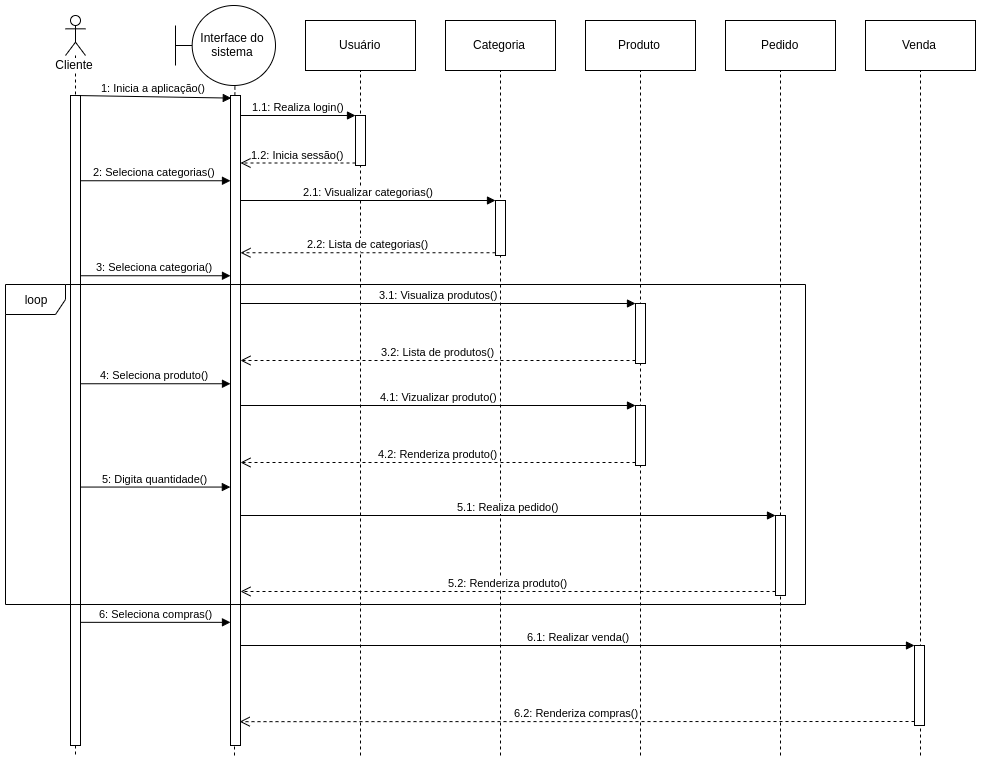
\includegraphics[width=1\textwidth]{figs/sequence3.png}
    \legend{Fonte: Elaborada pelo autor.}
    \label{fig:sequence3}
\end{figure}

\subsection{Diagrama de classes}
A figura \ref{fig:class} representa o diagrama de classes concebido para a aplicação. Todas as classes da aplicação serão derivadas da classe ApplicationRecord do \textit{framework} RoR, omitida nesse diagrama por conter inúmeros atributos e métodos genéricos, ficando assim inviável para apresentação.
\begin{figure}[htbp!]
  \centering
  \caption{Diagrama de classes}
  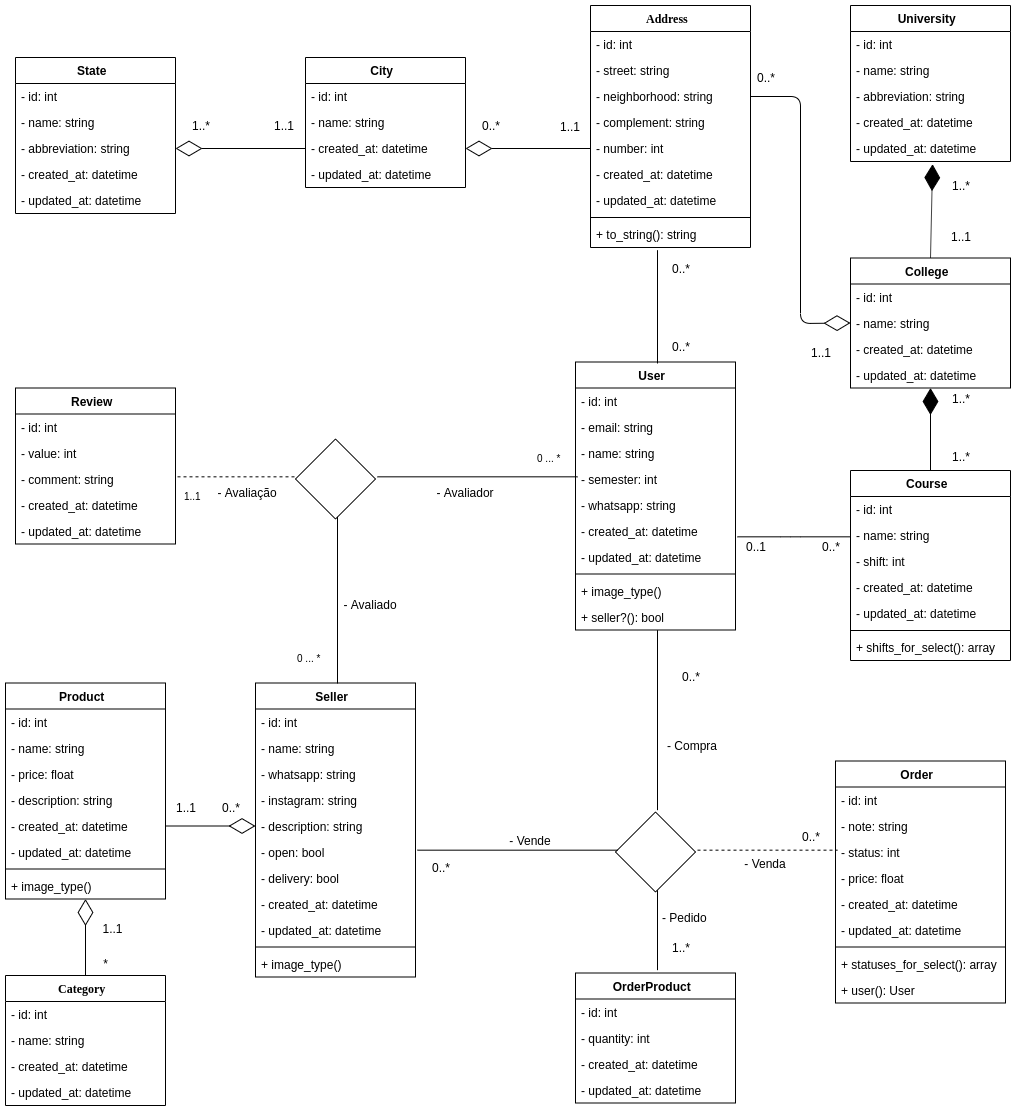
\includegraphics[width=1\textwidth]{figs/class.png}
    \legend{Fonte: Elaborada pelo autor.}
    \label{fig:class}
\end{figure}

\section{Versionamento do código}
% O processo de desenvolvimento do sistema utilizou desde o início várias ferramentas auxiliares. Software para versionamento de código, bibliotecas da linguagem, ferramenta de \textit{mockup}(como citada na seção \ref{mockup}) são algumas delas. Tais ferramentas contribuíram agilizar e facilitar o desenvolvimento do projeto.
% \subsection{Versionamento de código}
O objetivo mais básico dos softwares de controle de versão é armazenar e gerenciar o histórico de alterações feitas em um arquivo, dessa forma será possível retornar a versões anteriores do código caso seja necessário. No projeto aqui desenvolvido foi utilizado o versionador Git. O Git pode se conectar com várias plataformas online, como por exemplo o Github, Gitlab e outros para que o código fonte seja disponibilizado para o público.

\chapter{Resultados e discussões}
\label{chap:resultados}

Lorem ipsum dolor sit amet, consectetur adipiscing elit. Vivamus eu magna cursus, mattis velit et, pulvinar lorem. Integer ut nulla eget tellus luctus pellentesque. Nullam fermentum arcu sed tristique congue. Sed ut augue a turpis imperdiet maximus vitae accumsan nisi. Fusce vitae dapibus orci. Pellentesque rutrum tincidunt turpis, id blandit libero lacinia eu. Nunc imperdiet dolor scelerisque ex tristique, nec elementum sem iaculis.


\section{Testes automatizados}\label{tdd}
Esta seção avalia de forma sistemática toda a implementação técnica desenvolvida até o momento, busca uma melhor eficiência e qualidade do código da aplicação. Serão realizados quatro tipos de testes automatizados no Mercado Universitário. Testes unitários e integração, testes de segurança e testes de qualidade do código, tais testes serão apresentados a seguir.
\subsection{Testes unitários e integração}
Foi utilizada a gem RSpec para esse tipo de teste. Tal ferramenta foi apresentada na seção \ref{rspec}. De acordo com a imagem \ref{fig:rspec} foram realizados 102 exemplos de testes na aplicação, tais testes conseguiram cobrir 92.9\% de todo o código da aplicação sem que ocorresse nenhuma falha. Tal resultado se mostra bastante satisfatório, uma vez que se aproxima bastante de 100\% de cobertura do código e não apresenta nenhuma falha.
\begin{figure}[htbp!]
  \centering
  \caption{Saída do terminal para teste automatizado unitário e de integração utilizando a \textit{gem} RSpec}
  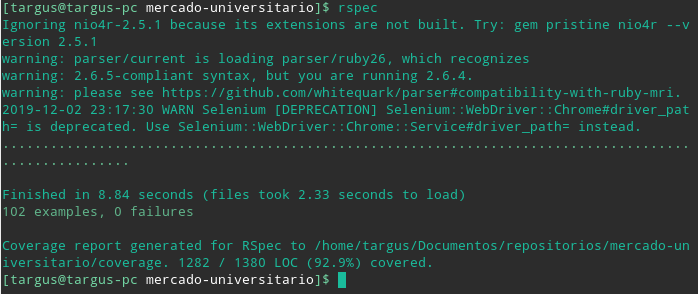
\includegraphics[width=1\textwidth]{figs/rspec.png}
    \legend{Fonte: Elaborada pelo autor.}
    \label{fig:rspec}
\end{figure}
\subsection{Testes de segurança}
Foram utilizadas duas \textit{gems} para realizar esse teste de grande importância para a aplicação. A \textit{gem} Brakeman em conjunto com a \textit{gem} Bundle Audit são suficientes para explorar as principais vulnerabilidades das aplicações web. Como é observado nas imagens \ref{fig:brakeman} e \ref{fig:audit}, não foram encontradas nenhuma vulnerabilidade na aplicação.
\begin{figure}[htbp!]
  \centering
  \caption{Saída do terminal para teste automatizado de segurança utilizando a \textit{gem} Brakeman}
  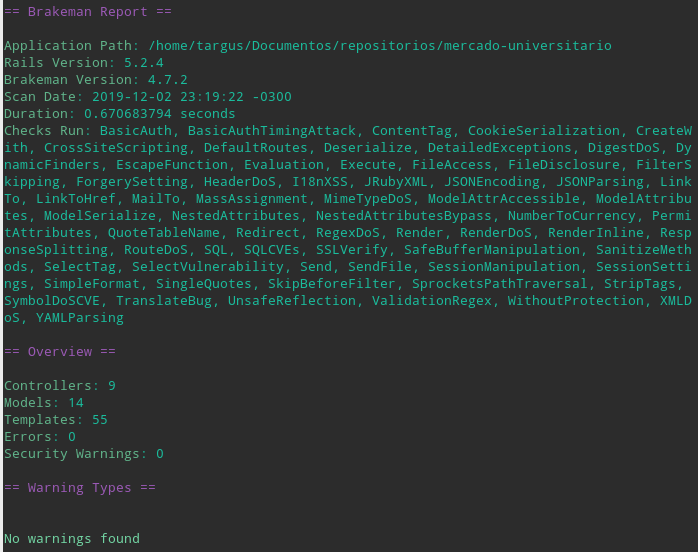
\includegraphics[width=1\textwidth]{figs/brakeman.png}
    \legend{Fonte: Elaborada pelo autor.}
    \label{fig:brakeman}
\end{figure}
\begin{figure}[htbp!]
  \centering
  \caption{Saída do terminal para teste automatizado de segurança utilizando a \textit{gem} Bundle Audit}
  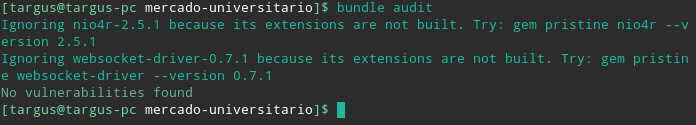
\includegraphics[width=1\textwidth]{figs/bundle_audit.png}
    \legend{Fonte: Elaborada pelo autor.}
    \label{fig:audit}
\end{figure}
\subsection{Testes de qualidade do código}
Para ser possível garantir uma boa manutenção e legibilidade futura do código, foi necessário utilizar a \textit{gem} Rubocop(apresentada na seção \ref{rubocop}). Como observado na imagem \ref{fig:rubocop}, foram verificadas as boas práticas de programação determinadas pelo Rails em 71 arquivos do projeto, não foi encontrada nenhuma ofensa no código.
\begin{figure}[htbp!]
  \centering
  \caption{Saída do terminal para verificação da qualidade do código utilizando a gem Rubocop}
  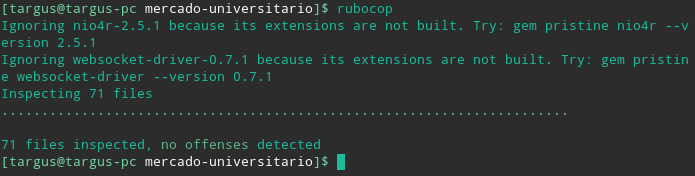
\includegraphics[width=1\textwidth]{figs/rubocop.png}
    \legend{Fonte: Elaborada pelo autor.}
    \label{fig:rubocop}
\end{figure}

\chapter{{Conteúdo aqui, conteúdo aqui}}
\label{chap:extracao_amendoas}

Lorem ipsum dolor sit amet, consectetur adipiscing elit. Vivamus eu magna cursus, mattis velit et, pulvinar lorem. Integer ut nulla eget tellus luctus pellentesque. Nullam fermentum arcu sed tristique congue. Sed ut augue a turpis imperdiet maximus vitae accumsan nisi. Fusce vitae dapibus orci. Pellentesque rutrum tincidunt turpis, id blandit libero lacinia eu. Nunc imperdiet dolor scelerisque ex tristique, nec elementum sem iaculis. Suspendisse eu leo sapien. Vivamus facilisis ultrices sollicitudin. Nunc suscipit, velit eget pretium rhoncus, erat nisl facilisis nulla, quis ultricies orci tellus sed ante. Sed pellentesque, nisl ac venenatis feugiat, augue enim consequat augue, sed porttitor sem purus in enim. Praesent vel tellus eu libero vehicula sodales. Integer tincidunt faucibus sollicitudin. Sed dapibus convallis metus, vel accumsan sem convallis ut.

\section{Metodologia proposta}
\label{sec:metodologia_proposta}

Lorem ipsum dolor sit amet, consectetur adipiscing elit. Vivamus eu magna cursus, mattis velit et, pulvinar lorem. Integer ut nulla eget tellus luctus pellentesque. Nullam fermentum arcu sed tristique congue. Sed ut augue a turpis imperdiet maximus vitae accumsan nisi. Fusce vitae dapibus orci. Pellentesque rutrum tincidunt turpis, id blandit libero lacinia eu. Nunc imperdiet dolor scelerisque ex tristique, nec elementum sem iaculis. Suspendisse eu leo sapien. Vivamus facilisis ultrices sollicitudin. Nunc suscipit, velit eget pretium rhoncus, erat nisl facilisis nulla, quis ultricies orci tellus sed ante. Sed pellentesque, nisl ac venenatis feugiat, augue enim consequat augue, sed porttitor sem purus in enim. Praesent vel tellus eu libero vehicula sodales. Integer tincidunt faucibus sollicitudin. Sed dapibus convallis metus, vel accumsan sem convallis ut.
% \chapter{Testes e resultados}

Lorem ipsum dolor sit amet, consectetur adipiscing elit. Vivamus eu magna cursus, mattis velit et, pulvinar lorem. Integer ut nulla eget tellus luctus pellentesque. Nullam fermentum arcu sed tristique congue. Sed ut augue a turpis imperdiet maximus vitae accumsan nisi. Fusce vitae dapibus orci. Pellentesque rutrum tincidunt turpis, id blandit libero lacinia eu. Nunc imperdiet dolor scelerisque ex tristique, nec elementum sem iaculis. Suspendisse eu leo sapien. Vivamus facilisis ultrices sollicitudin. Nunc suscipit, velit eget pretium rhoncus, erat nisl facilisis nulla, quis ultricies orci tellus sed ante. Sed pellentesque, nisl ac venenatis feugiat, augue enim consequat augue, sed porttitor sem purus in enim. Praesent vel tellus eu libero vehicula sodales. Integer tincidunt faucibus sollicitudin. Sed dapibus convallis metus, vel accumsan sem convallis ut.

\section{Passo 1}

Lorem ipsum dolor sit amet, consectetur adipiscing elit. Vivamus eu magna cursus, mattis velit et, pulvinar lorem. Integer ut nulla eget tellus luctus pellentesque. Nullam fermentum arcu sed tristique congue. Sed ut augue a turpis imperdiet maximus vitae accumsan nisi. Fusce vitae dapibus orci. Pellentesque rutrum tincidunt turpis, id blandit libero lacinia eu. Nunc imperdiet dolor scelerisque ex tristique, nec elementum sem iaculis. Suspendisse eu leo sapien. Vivamus facilisis ultrices sollicitudin. Nunc suscipit, velit eget pretium rhoncus, erat nisl facilisis nulla, quis ultricies orci tellus sed ante. Sed pellentesque, nisl ac venenatis feugiat, augue enim consequat augue, sed porttitor sem purus in enim. Praesent vel tellus eu libero vehicula sodales.

\section{Passo 2}

Lorem ipsum dolor sit amet, consectetur adipiscing elit. Vivamus eu magna cursus, mattis velit et, pulvinar lorem. Integer ut nulla eget tellus luctus pellentesque. Nullam fermentum arcu sed tristique congue. Sed ut augue a turpis imperdiet maximus vitae accumsan nisi. Fusce vitae dapibus orci. Pellentesque rutrum tincidunt turpis, id blandit libero lacinia eu. Nunc imperdiet dolor scelerisque ex tristique, nec elementum sem iaculis. Suspendisse eu leo sapien. Vivamus facilisis ultrices sollicitudin. Nunc suscipit, velit eget pretium rhoncus, erat nisl facilisis nulla, quis ultricies orci tellus sed ante. Sed pellentesque, nisl ac venenatis feugiat, augue enim consequat augue, sed porttitor sem purus in enim. Praesent vel tellus eu libero vehicula sodales. Integer tincidunt faucibus sollicitudin. Sed dapibus convallis metus, vel accumsan sem convallis ut.

\section{Passo 3}

Lorem ipsum dolor sit amet, consectetur adipiscing elit. Vivamus eu magna cursus, mattis velit et, pulvinar lorem. Integer ut nulla eget tellus luctus pellentesque. Nullam fermentum arcu sed tristique congue. Sed ut augue a turpis imperdiet maximus vitae accumsan nisi. Fusce vitae dapibus orci. Pellentesque rutrum tincidunt turpis, id blandit libero lacinia eu. Nunc imperdiet dolor scelerisque ex tristique, nec elementum sem iaculis. Suspendisse eu leo sapien. Vivamus facilisis ultrices sollicitudin. Nunc suscipit, velit eget pretium rhoncus, erat nisl facilisis nulla, quis ultricies orci tellus sed ante. Sed pellentesque, nisl ac venenatis feugiat, augue enim consequat augue, sed porttitor sem purus in enim. Praesent vel tellus eu libero vehicula sodales. Integer tincidunt faucibus sollicitudin. Sed dapibus convallis metus, vel accumsan sem convallis ut.

Sed dapibus convallis metus, vel accumsan sem convallis ut em \textit{img\_i} vel accumsan sem convallis. Lorem ipsum dolor sit amet, consectetur adipiscing elit. Vivamus eu magna cursus, mattis velit et, pulvinar lorem. A Figura X apresenta o resultado obtido com \textit{img\_i}.

\section{Passo 4}

Lorem ipsum dolor sit amet, consectetur adipiscing elit. Vivamus eu magna cursus, mattis velit et, pulvinar lorem. Integer ut nulla eget tellus luctus pellentesque. Nullam fermentum arcu sed tristique congue. Sed ut augue a turpis imperdiet maximus vitae accumsan nisi. Fusce vitae dapibus orci. Pellentesque rutrum tincidunt turpis, id blandit libero lacinia eu. Nunc imperdiet dolor scelerisque ex tristique, nec elementum sem iaculis. Suspendisse eu leo sapien. Vivamus facilisis ultrices sollicitudin. Nunc suscipit, velit eget pretium rhoncus, erat nisl facilisis nulla, quis ultricies orci tellus sed ante. Sed pellentesque, nisl ac venenatis feugiat, augue enim consequat augue, sed porttitor sem purus in enim. Praesent vel tellus eu libero vehicula sodales. Integer tincidunt faucibus sollicitudin. Sed dapibus convallis metus, vel accumsan sem convallis ut.

\section{Passo 5}

Lorem ipsum dolor sit amet, consectetur adipiscing elit. Vivamus eu magna cursus, mattis velit et, pulvinar lorem. Integer ut nulla eget tellus luctus pellentesque. Nullam fermentum arcu sed tristique congue. Sed ut augue a turpis imperdiet maximus vitae accumsan nisi. Fusce vitae dapibus orci. Pellentesque rutrum tincidunt turpis, id blandit libero lacinia eu. Nunc imperdiet dolor scelerisque ex tristique, nec elementum sem iaculis. Suspendisse eu leo sapien. Vivamus facilisis ultrices sollicitudin. Nunc suscipit, velit eget pretium rhoncus, erat nisl facilisis nulla, quis ultricies orci tellus sed ante. Sed pellentesque, nisl ac venenatis feugiat, augue enim consequat augue, sed porttitor sem purus in enim. Praesent vel tellus eu libero vehicula sodales. Integer tincidunt faucibus sollicitudin. Sed dapibus convallis metus, vel accumsan sem convallis ut.

\section{Passo 6}

Lorem ipsum dolor sit amet, consectetur adipiscing elit. Vivamus eu magna cursus, mattis velit et, pulvinar lorem. Integer ut nulla eget tellus luctus pellentesque. Nullam fermentum arcu sed tristique congue. Sed ut augue a turpis imperdiet maximus vitae accumsan nisi. Fusce vitae dapibus orci. Pellentesque rutrum tincidunt turpis, id blandit libero lacinia eu. Nunc imperdiet dolor scelerisque ex tristique, nec elementum sem iaculis. Suspendisse eu leo sapien. Vivamus facilisis ultrices sollicitudin. Nunc suscipit, velit eget pretium rhoncus, erat nisl facilisis nulla, quis ultricies orci tellus sed ante. Sed pellentesque, nisl ac venenatis feugiat, augue enim consequat augue, sed porttitor sem purus in enim. Praesent vel tellus eu libero vehicula sodales. Integer tincidunt faucibus sollicitudin. Sed dapibus convallis metus, vel accumsan sem convallis ut.
% \chapter{Conclusões e Trabalhos Futuros}
\label{chap:conclusoes_trabalhos_futuros}

Lorem ipsum dolor sit amet, consectetur adipiscing elit. Vivamus eu magna cursus, mattis velit et, pulvinar lorem. Integer ut nulla eget tellus luctus pellentesque. Nullam fermentum arcu sed tristique congue. Sed ut augue a turpis imperdiet maximus vitae accumsan nisi. Fusce vitae dapibus orci.

\section{Méritos e Limitações}

Lorem ipsum dolor sit amet, consectetur adipiscing elit. Vivamus eu magna cursus, mattis velit et, pulvinar lorem. Integer ut nulla eget tellus luctus pellentesque. Nullam fermentum arcu sed tristique congue. Sed ut augue a turpis imperdiet maximus vitae accumsan nisi. Fusce vitae dapibus orci. Pellentesque rutrum tincidunt turpis, id blandit libero lacinia eu. Nunc imperdiet dolor scelerisque ex tristique, nec elementum sem iaculis. Suspendisse eu leo sapien. Vivamus facilisis ultrices sollicitudin. Nunc suscipit, velit eget pretium rhoncus, erat nisl facilisis nulla, quis ultricies orci tellus sed ante. Sed pellentesque, nisl ac venenatis feugiat, augue enim consequat augue, sed porttitor sem purus in enim. Praesent vel tellus eu libero vehicula sodales. Integer tincidunt faucibus sollicitudin. Sed dapibus convallis metus, vel accumsan sem convallis ut.

% \subsection{Contribuições pessoais}
% O que o trabalho contribuiu para o seu aprendizado pessoal?

% ----------------------------------------------------------
% Finaliza a parte no bookmark do PDF
% para que se inicie o bookmark na raiz
% e adiciona espaço de parte no Sumário
% ----------------------------------------------------------
\phantompart

% ---
% Conclusão
% ---
%\chapter{Conclusão}
% ---

% ----------------------------------------------------------
% ELEMENTOS PÓS-TEXTUAIS
% ----------------------------------------------------------
\postextual
% ----------------------------------------------------------

% ----------------------------------------------------------
% Referências bibliográficas
% ----------------------------------------------------------
\bibliography{TCC.bib}

% ----------------------------------------------------------
% Glossário
% ----------------------------------------------------------
%
% Consulte o manual da classe abntex2 para orientações sobre o glossário.
%
%\glossary

% ----------------------------------------------------------
% Apêndices
% ----------------------------------------------------------

% ---
% Inicia os apêndices
% ---
\begin{apendicesenv}

% Imprime uma página indicando o início dos apêndices
\partapendices

% ----------------------------------------------------------
\chapter{Lista de todos os requisitos funcionais do sistema}
% ----------------------------------------------------------

Devido a grande quantidade, foi preciso apresentar nos apêndices a lista contendo todos os requisitos funcionais do sistema Mercado Universitário. Segue abaixo a lista.

\textbf{RF01 - Cadastrar usuário} \par
\textbf{Prioridade:} Essencial \par
\textbf{Atores:} Convidado \par
\textbf{Descrição:} Qualquer pessoa que acessa o sistema, seja um discente, funcionário, professor, ou pessoas que vivem no âmbito universitário podem se cadastrar no sistema como um cliente por meio do formulário público que se encontra na página inicial da aplicação. Será necessário que o ator convidado preencha corretamente os dados obrigatórios cumprindo suas respectivas validações, caso contrário o próprio sistema irá apontar o erro para ser sanado. \par
\textbf{Fluxo de eventos:} \par
\textbf{Principal} \par
\begin{enumerate}
  \item O ator insere as informações de cadastro solicitadas, como email, senha, nome, universidade, curso, whatsapp e foto de perfil.
  \item O sistema fará login automaticamente no sistema informando que o usuário foi cadastrado com sucesso.
\end{enumerate} \par
\textbf{Secundário} \par
\begin{enumerate}
  \item O ator insere as informações de cadastro solicitadas, como email, senha, nome, universidade, curso, whatsapp e foto de perfil.
  \item O sistema renderiza a mesma página informando que os dados submetidos não foram cumprem algumas validações e identifica onde está os erros no formulário.
  \item O ator corrige os dados e submete novamente o cadastro para o sistema.
\end{enumerate}

\textbf{RF02 - Fazer login} \par
\textbf{Prioridade:} Essencial \par
\textbf{Atores:} Cliente \par
\textbf{Descrição:} Após realizar o cadastro, o usuário estará apto a fazer o login na plataforma para ter acesso a todo o ambiente que o sistema proporciona. O login é totalmente essencial por ter a capacidade de identificar unicamente cada usuário do sistema por meio do seu e-mail e senha, fazendo assim com que o resto do sistema traga informações relativas em relação aquele ator que acabou de logar, como por exemplo retornar apenas compras realizadas pelo ator logado. \par
\textbf{Fluxo de eventos:} \par
\textbf{Principal} \par
\begin{enumerate}
  \item O usuário insere suas credenciais(e-mail e senha) e clica no botão para logar
  \item O sistema redireciona para a página de produtos e informa que o login foi bem sucedido.
\end{enumerate}

\textbf{RF03 - Visualizar categorias dos produtos} \par
\textbf{Prioridade:} Essencial \par
\textbf{Atores:} Cliente \par
\textbf{Descrição:} Todos os produtos da aplicação estão atrelados a uma categoria específica, isso facilita bastante a busca por um determinado item. Existirá diversas categorias, como por exemplo, alimentos, roupas, acessórios, bebidas, dentre outros. É possível filtrar a lista de categorias por meio de pesquisa. \par
\textbf{Fluxo de eventos:} \par
\textbf{Principal} \par
\begin{enumerate}
  \item O usuário seleciona a opção “categorias” por meio do navbar da aplicação.
  \item O sistema direciona para uma página mostrando as categorias do sistema não extrapolando o limite máximo determinado pela paginação.
\end{enumerate} \par
\textbf{Secundário} \par
\begin{enumerate}
  \item O usuário seleciona a opção “categorias” por meio do navbar da aplicação.
  \item Por meio da caixa de pesquisa o usuário digita o nome(ou parte dele) da categoria que deseja buscar.
  \item A mesma página é renderizada mostrando apenas as categorias que condizem com a palavra-chave digitada pelo usuário.
\end{enumerate}

\textbf{RF04 - Visualizar lista vendedores} \par
\textbf{Prioridade:} Essencial \par
\textbf{Atores:} Cliente \par
\textbf{Descrição:} Todos os vendedores que realizam entregas/vendas na mesma universidade em que o cliente se encontra serão listados. Facilitando assim explorar os diversos vendedores que atuam na universidade. É possível filtrar a lista de vendedores por meio de pesquisa. \par
\textbf{Fluxo de eventos:} \par
\textbf{Principal} \par
\begin{enumerate}
  \item O usuário seleciona a opção “vendedores” por meio do navbar da aplicação.
  \item O sistema direciona para uma página mostrando todos os vendedores da universidade, não extrapolando o limite máximo determinado pela paginação.
\end{enumerate} \par
\textbf{Secundário} \par
\begin{enumerate}
  \item O usuário seleciona a opção “vendedores” por meio do navbar da aplicação.
  \item Por meio da caixa de pesquisa o usuário digita o nome(ou parte dele) do vendedor que pretende buscar.
  \item A mesma página é renderizada mostrando apenas os vendedores que condizem com a palavra-chave digitada pelo usuário e que atuam na universidade do usuário.
\end{enumerate}

\textbf{RF05 - Visualizar lista de produtos} \par
\textbf{Prioridade:} Essencial \par
\textbf{Atores:} Cliente e Vendedor \par
\textbf{Descrição:} O sistema deve ser capaz de listar os produtos relacionado ao ator em questão. Pode ser uma listagem de todos os produtos da universidade, todos os produtos de uma categoria específica, ou todos os produtos de um vendedor específico. Não será possível ser listado que um vendedor consiga listar produtos de outros vendedores. \par
\textbf{Fluxo de eventos:} \par
\textbf{Principal} \par
\begin{enumerate}
  \item O cliente seleciona a uma categoria de produtos.
  \item Será listado todos os produtos da universidade do cliente que sejam da categoria selecionada.
\end{enumerate}

\textbf{RF06 - Visualizar produto} \par
\textbf{Prioridade:} Essencial \par
\textbf{Atores:} Cliente e Vendedor \par
\textbf{Descrição:} Será possível a visualização de um produto específico de um determinado vendedor, mostrando sua foto e descrição, bem como a opção de adicionar este produto ao carrinho de compras. Caso o ator seja um vendedor, aparecerá a opção de editar ou remover o produto em questão. \par
\textbf{Fluxo de eventos:} \par
\textbf{Principal} \par
\begin{enumerate}
  \item O ator escolherá um produto específico a partir de uma lista.
  \item Será direcionado para a página específica do produto.
  \item O ator visualiza o produto e poderá interagir com ele de acordo com seu perfil.
\end{enumerate}

\textbf{RF07 - Visualizar vendedor} \par
\textbf{Prioridade:} Essencial \par
\textbf{Atores:} Cliente e Vendedor \par
\textbf{Descrição:} O cliente conseguirá acessar a página específica de qualquer vendedor da sua universidade, nesta página será possível ter acesso ao instagram, whatsapp, descrição, se faz entrega ou não, se está aberto ou não, e reviews do vendedor em questão. Todavia, caso o ator seja um vendedor, ele só poderá acessar sua própria página. \par
\textbf{Fluxo de eventos:} \par
\textbf{Principal} \par
\begin{enumerate}
  \item O cliente clica em um dos vendedores da lista de vendedores da sua universidade.
  \item Será redirecionado para a página específica do vendedor que clicou.
  \item Nesta página terá acesso ao dados do vendedor.
\end{enumerate}

\textbf{RF08 - Cadastrar \textit{review} de um vendedor} \par
\textbf{Prioridade:} Essencial \par
\textbf{Atores:} Cliente \par
\textbf{Descrição:} O cliente poderá compartilhar sua opinião acerca de algum vendedor por meio da página de cadastro de \textit{review}, colocando em um formulário a descrição e nota(entre 1 e 5, inclusos) do vendedor. \par
\textbf{Fluxo de eventos:} \par
\textbf{Principal} \par
\begin{enumerate}
  \item O cliente acessa a página específica do vendedor
  \item Clica no link “deixe sua opinião!”
  \item Será redirecionado para página de cadastro de \textit{review}
  \item Preenche o formulário
  \item Submete os dados
  \item Será redirecionado para página do vendedor informando que a operação foi bem sucedida
\end{enumerate}

\textbf{RF09 - Atualizar review de um vendedor} \par
\textbf{Prioridade:} Essencial \par
\textbf{Atores:} Cliente \par
\textbf{Descrição:} Apenas o cliente que cadastrou o review poderá atualizá-lo. O formulário será o mesmo utilizado para cadastrar, porém dessa vez será realizada uma operação de atualização. \par
\textbf{Fluxo de eventos:} \par
\textbf{Principal} \par
\begin{enumerate}
  \item O cliente acessa a página do vendedor ao qual deseja atualizar seu review.
  \item Clica no link “edite sua opinião”.
  \item Será redirecionado para página de editar review.
  \item Altera seu review no formulário.
  \item Submete os novos dados.
  \item Será redirecionado para página do vendedor sendo informado que a operação foi bem sucedida.
\end{enumerate}

\textbf{RF10 - Adicionar produto ao carrinho de compras} \par
\textbf{Prioridade:} Essencial \par
\textbf{Atores:} Cliente \par
\textbf{Descrição:} Para compor um pedido, é necessário adicionar produtos ao pedido. O cliente poderá fazer isso diretamente na página do produto em que deseja comprar, colocando assim a quantidade desejada e clicando em “adicionar produto”. \par
\textbf{Fluxo de eventos:} \par
\textbf{Principal} \par
\begin{enumerate}
  \item Na página do produto, o cliente insere a quantidade do produto para ser adicionado
  \item Clica em “adicionar produto“
  \item Será redirecionado para página de produto com a notificação informando que a operação foi bem sucedida
\end{enumerate}

\textbf{RF11 - Visualizar pedidos} \par
\textbf{Prioridade:} Essencial \par
\textbf{Atores:} Cliente e vendedor \par
\textbf{Descrição:} Por meio do link “meus pedidos” na navbar será possível visualizar a lista de pedidos feitos(já realizados e que estão a realizar) pelo cliente. O vendedor conseguirá acessar a página pelo mesmo link do cliente, entretanto será mostrado apenas os pedidos já recebidos pelo vendedor, independentemente do status da compra ao qual o pedido se encontra. \par
\textbf{Fluxo de eventos:} \par
\textbf{Principal} \par
\begin{enumerate}
  \item O cliente acessa a página de pedidos pelo link do navbar
  \item Será renderizado duas sessões de lista de pedidos: pedidos já realizados e pedidos em aberto
  \item O cliente terá a opção de realizar os pedidos em aberto
\end{enumerate}

\textbf{RF12 - Cadastrar conta de vendedor} \par
\textbf{Prioridade:} Essencial \par
\textbf{Atores:} Cliente \par
\textbf{Descrição:} Para se tornar um vendedor, necessariamente é preciso que o ator seja um cliente, para então realizar o devido cadastro da conta. Só será possível uma conta de vendedor para cada conta cliente. O link denominado “seja um vendedor” para cadastro da conta estará disponível no navbar da aplicação. \par
\textbf{Fluxo de eventos:} \par
\textbf{Principal} \par
\begin{enumerate}
  \item O cliente clica no link “seja um vendedor” no navbar
  \item Será redirecionado para a página com um formulário para inserir os dados do vendedor
  \item Preenche os campos
  \item Submete os dados para ser cadastrado no banco de dados
  \item É redirecionado para a área restrita sendo informado que o cadastro foi realizado com sucesso
\end{enumerate}

\textbf{RF13 - Acessar área restrita} \par
\textbf{Prioridade:} Essencial \par
\textbf{Atores:} Vendedor \par
\textbf{Descrição:} Ao realizar o login na aplicação, o usuário acessa automaticamente a área do cliente. Se o cliente tem uma conta de vendedor, aparecerá um link denominado “Área restrita” na navbar, no mesmo local onde aparece “seja um vendedor” para os  clientes que não tem uma conta de vendedor. Ao clicar neste link, o ator será redirecionado para a área restrita para vendedores, onde poderá administrar os produtos e controle de produtos. \par
\textbf{Fluxo de eventos:} \par
\textbf{Principal} \par
\begin{enumerate}
  \item O ator clica no link “Área restrita”
  \item Será redirecionado para a página de produtos da área restrita
\end{enumerate}

\textbf{RF14 - Cadastrar produto} \par
\textbf{Prioridade:} Essencial \par
\textbf{Atores:} Vendedor \par
\textbf{Descrição:} Como o intuito básico da aplicação será venda de produtos, será possível que cada vendedor insira seus produtos na plataforma por meio de um formulário, informando o nome, descrição, valor e foto do produto em questão. \par
\textbf{Fluxo de eventos:} \par
\textbf{Principal} \par
\begin{enumerate}
  \item Na página de listagem dos seus produtos, o vendedor clicará no link “Inserir novo produto”.
  \item Será redirecionado para a página que contém o formulário.
  \item Preenche todos os campos.
  \item Submete o formulário.
  \item Será redirecionado para a página do produto criado sendo informado que a operação foi concluída com sucesso.
\end{enumerate} \par
\textbf{Secundário} \par
\begin{enumerate}
  \item Na página de listagem dos seus produtos, o vendedor clicará no link “Inserir novo produto”.
  \item Será redirecionado para a página que contém o formulário.
  \item Preenche todos os campos.
  \item Submete o formulário.
  \item A mesma página é renderizada informando que contém campos inválidos no formulário.
  \item O vendedor corrige os campos inválidos e submete novamente.
\end{enumerate}

\textbf{RF15 - Editar produto} \par
\textbf{Prioridade:} Essencial \par
\textbf{Atores:} Vendedor \par
\textbf{Descrição:} Quando o vendedor possui produtos cadastrados, é possível editá-los facilmente. Para isso é preciso acessar a página do produto a ser editado e clicar no link “editar”. Cada vendedor poderá editar apenas seus próprios produtos. \par
\textbf{Fluxo de eventos:} \par
\textbf{Principal} \par
\begin{enumerate}
  \item O vendedor acessa a página do produto a ser editado.
  \item Clica no link “Editar”.
  \item Será redirecionado para página que contém o formulário.
  \item Altera os dados que desejar.
  \item Submete as alterações do formulário.
  \item Será redirecionado para a página do produto sendo informado que as alterações foram efetivadas.
\end{enumerate} \par
\textbf{Secundário} \par
\begin{enumerate}
  \item O vendedor acessa a página do produto a ser editado.
  \item Clica no link “Editar”.
  \item Será redirecionado para página que contém o formulário.
  \item Altera os dados que desejar.
  \item Submete as alterações do formulário.
  \item Será renderizada a mesma página sendo informado que existem dados inválidos.
  \item O vendedor corrige os dados inválidos e submete novamente o formulário.
\end{enumerate}

\textbf{RF16 - Realizar pedido de compra} \par
\textbf{Prioridade:} Essencial \par
\textbf{Atores:} Cliente \par
\textbf{Descrição:} O ato de realizar o pedido é um recurso fundamental para a aplicação. Este requisito efetua a conexão entre um cliente e o vendedor(que no caso seria o fornecedor dos produtos do pedido em questão). Nessa etapa será possível deixar um recado para o vendedor e selecionar o local de entrega(caso o vendedor realize entregas). \par
\textbf{Fluxo de eventos:} \par
\textbf{Principal} \par
\begin{enumerate}
  \item O cliente clicará no link “meus pedidos” no navbar
  \item Será redirecionado para a página com a lista de pedidos fechados e abertos
  \item Preencherá um recado para o vendedor
  \item Escolherá o tipo de entrega/local do pedido
  \item Realiza o pedido clicando no botão “realizar pedido”
  \item Será renderizada a mesma página informando que o pedido foi efetivado
\end{enumerate}

\textbf{RF17 - Atualizar status do pedido} \par
\textbf{Prioridade:} Essencial \par
\textbf{Atores:} Vendedor \par
\textbf{Descrição:} O controle do status da compra é útil para que o cliente saiba em qual etapa seu pedido se encontra, são elas: não visto, preparando, a caminho, entregue, cancelado. O vendedor deverá alterar esse status de maneira condizente. Esse controle de status também facilitará a organização do vendedor, sendo que fica mais fácil o controle de todos seus pedidos correntes. \par
\textbf{Fluxo de eventos:} \par
\textbf{Principal} \par
\begin{enumerate}
  \item O vendedor clica no link “meus pedidos” na navbar.
  \item Será redirecionado para a página listando os pedidos.
  \item O vendedor altera o status de algum pedido da lista por meio select.
  \item A mesma página será renderizada informando que o status foi alterado.
\end{enumerate}

\textbf{RF18 - Visualizar usuários} \par
\textbf{Prioridade:} Essencial \par
\textbf{Atores:} Vendedor \par
\textbf{Descrição:} Para uma maior eficácia na entrega dos pedidos, é necessário que o vendedor tenha informações básicas sobre o cliente que fez o pedido. Essas informações básicas podem ser obtidas por meio da página individual do cliente, a qual contém informações como: foto, nome, curso, semestre e whatsapp do cliente. \par
\textbf{Fluxo de eventos:} \par
\textbf{Principal} \par
\begin{enumerate}
  \item O vendedor clica no link com o nome do cliente que está página de lista de pedidos.
  \item Será redirecionado para a página individual do cliente.
\end{enumerate}

\textbf{RF19 - Recuperar senha do login} \par
\textbf{Prioridade:} Importante \par
\textbf{Atores:} Cliente \par
\textbf{Descrição:} Para que não seja impossibilitado o acesso ao sistema pelo motivo de ter esquecido a senha de login, se mostra importante o mecanismo automatizado para recuperar as senhas. Diante disso, o sistema contará com essa facilidade, bastando colocar o email de recuperação e um link para geração da nova senha ser enviado para o email da pessoa solicitante. \par
\textbf{Fluxo de eventos:} \par
\textbf{Principal} \par
\begin{enumerate}
  \item O usuário acessa a página inicial.
  \item Clica no link de recuperação de senha.
  \item Solicita recuperação com seu email.
  \item Clica no link recebido no seu email.
  \item Cadastra a nova senha.
\end{enumerate}

\textbf{RF20 - Confirmação de recebimento da entrega} \par
\textbf{Prioridade:} Importante \par
\textbf{Atores:} Cliente \par
\textbf{Descrição:} É importante que os clientes confirmem o recebimento de entrega dos produtos, isso ajudará o controle interno do vendedor, bem como o próprio cliente futuramente. Esse função estará disponível na página de pedidos do sistema, bastando um clique para confirmar recebimento em pedidos que constam com o status “entregue”. \par
\textbf{Fluxo de eventos:} \par
\textbf{Principal} \par
\begin{enumerate}
  \item O cliente acessa a página de pedidos.
  \item Localiza o pedido com status “entregue” cadastrado pelo vendedor.
  \item Clica no botão de confirmação.
  \item A página será novamente renderizada com o pedido confirmado.
\end{enumerate}

\textbf{RF21 - Línguas estrangeiras} \par
\textbf{Prioridade:} Desejável \par
\textbf{Atores:} Cliente e Vendedor \par
\textbf{Descrição:} Por ter um nicho universitário, muitas das vezes pessoas de outros países tem contato com esse âmbito, pessoas essas que podem não falar o idioma português. Dessa forma, é desejável que o sistema seja bilíngue, suportando o idioma nativo(português) e um idioma bastante difundido(inglês). A mudança de idioma ocorrerá a qualquer momento de uso do sistema, bastando um clique para que os textos estáticos da aplicação alterne entre tais idiomas. \par
\textbf{Fluxo de eventos:} \par
\textbf{Principal} \par
\begin{enumerate}
  \item O usuário acessa a aplicação
  \item Clica na bandeira referente ao idioma desejado
  \item A página é renderizada com o novo idioma
\end{enumerate}

% \lipsum[50]

% ----------------------------------------------------------
% \chapter{Nullam elementum urna vel imperdiet sodales elit ipsum pharetra ligula
% ac pretium ante justo a nulla curabitur tristique arcu eu metus}
% % ----------------------------------------------------------
% \lipsum[55-57]

\end{apendicesenv}
% ---

%% ----------------------------------------------------------
% Anexos
% ----------------------------------------------------------

% ---
% Inicia os anexos
% ---
\begin{anexosenv}

% Imprime uma página indicando o início dos anexos
\partanexos

% ---
\chapter{Imagens resultantes da erosão e dilatação}
% ---

A seguir são apresentados as imagens resultantes da aplicação da erosão seguida da dilatação para as outras classes.

\begin{figure}[hbtp!]
 \centering
 \caption{Passo 3.2: Erosão e Dilatação na classe achatada}
 \includegraphics[scale=0.26]{figs/passos/passo_3/erode_dilate/passo_3_achatada.png}
 \legend{Fonte: Elaborada pelo autor}
 \label{fig:passo_3.2_achatada}
\end{figure}

\begin{figure}[hbtp!]
 \centering
 \caption{Passo 3.2: Erosão e Dilatação na classe germinada}
 \includegraphics[scale=0.26]{figs/passos/passo_3/erode_dilate/passo_3_germinada.png}
 \legend{Fonte: Elaborada pelo autor}
 \label{fig:passo_3.2_germinada}
\end{figure}

\begin{figure}[hbtp!]
 \centering
 \caption{Passo 3.2: Erosão e Dilatação na classe inseto}
 \includegraphics[scale=0.26]{figs/passos/passo_3/erode_dilate/passo_3_inseto.png}
 \legend{Fonte: Elaborada pelo autor}
 \label{fig:passo_3.2_inseto}
\end{figure}

\begin{figure}[hbtp!]
 \centering
 \caption{Passo 3.2: Erosão e Dilatação na classe parc. marrom}
 \includegraphics[scale=0.26]{figs/passos/passo_3/erode_dilate/passo_3_parc_marrom.png}
 \legend{Fonte: Elaborada pelo autor}
 \label{fig:passo_3.2_parc_marrom}
\end{figure}

\begin{figure}[hbtp!]
 \centering
 \caption{Passo 3.2: Erosão e Dilatação na classe marrom}
 \includegraphics[scale=0.26]{figs/passos/passo_3/erode_dilate/passo_3_marrom.png}
 \legend{Fonte: Elaborada pelo autor}
 \label{fig:passo_3.2_marrom}
\end{figure}

\begin{figure}[hbtp!]
 \centering
 \caption{Passo 3.2: Erosão e Dilatação na classe violeta}
 \includegraphics[scale=0.26]{figs/passos/passo_3/erode_dilate/passo_3_violeta.png}
 \legend{Fonte: Elaborada pelo autor}
 \label{fig:passo_3.2_violeta}
\end{figure}

\newpage
% ---
\chapter{Tabelas de características geométricas}
% ---
As Tabelas(\ref{tab:medidas_classe_achatada}, \ref{tab:medidas_classe_ardosia}, \ref{tab:medidas_classe_germinada}, \ref{tab:medidas_classe_inseto}, \ref{tab:medidas_classe_parc_marrom}, \ref{tab:medidas_classe_marrom} e \ref{tab:medidas_classe_violeta}) apresentam as características geométricas extraídas das classes de amêndoas.

\begin{table}[hbtp!]
\centering
\caption{Comparação de medidas da amêndoa da classe achatada}
\label{tab:medidas_classe_achatada}
\begin{tabular}{|l|l|l|l|l|l|l|l|}
\hline
Nº & 2/5 & 3/5 & 4/5 & Larg. Média & Área & Nº de amostras & Acima da Média (Larg.) \\ \hline
1  & 15  & 15  & 12  & 14          & 449  & 20               & 8                      \\
2  & 10  & 11  & 9   & 10          & 300  &                  &                        \\\cline{7-8}
3  & 14  & 16  & 13  & 14,3333     & 439  & \multicolumn{1}{l|}{Larg. 2/5 média}   & \multicolumn{1}{l|}{Abaixo da media (Larg.)} \\\cline{7-8}
4  & 12  & 13  & 10  & 11,6667     & 384  & 12,7             & 12                     \\
5  & 11  & 13  & 9   & 11          & 378  &                  &                        \\\cline{7-8}
6  & 11  & 19  & 17  & 15,6667     & 336  & \multicolumn{1}{l|}{Larg. 3/5 média}   & \multicolumn{1}{l|}{Acima da media (area)}  \\\cline{7-8}
7  & 12  & 13  & 13  & 12,6667     & 361  & 15,05            & 9                      \\
8  & 13  & 13  & 10  & 12          & 358  &                  &                        \\\cline{7-8}
9  & 18  & 18  & 12  & 16          & 575  & \multicolumn{1}{l|}{Larg. 4/5 média}   & \multicolumn{1}{l|}{Abaixo da media (area)} \\\cline{7-8}
10 & 14  & 19  & 13  & 15,3333     & 517  & 12,45            & 11                     \\
11 & 12  & 17  & 15  & 14,6667     & 487  &                  &                        \\\cline{7-8}
12 & 10  & 15  & 15  & 13,3333     & 443  & Larg. média total & \multicolumn{1}{l|}{Área média}             \\\cline{7-8}
13 & 10  & 14  & 14  & 12,6667     & 484  & 13,400005        & 439,7                  \\
14 & 11  & 15  & 13  & 13          & 449  &                  &                        \\
15 & 13  & 15  & 10  & 12,6667     & 408  &                  &                        \\
16 & 13  & 13  & 11  & 12,3333     & 391  &                  &                        \\
17 & 14  & 15  & 10  & 13          & 396  &                  &                        \\
18 & 14  & 15  & 11  & 13,3333     & 435  &                  &                        \\
19 & 13  & 17  & 17  & 15,6667     & 582  &                  &                        \\
20 & 14  & 15  & 15  & 14,6667     & 622  &                  &                       \\\hline
\end{tabular}
\legend{Fonte: Dados da pesquisa}
\end{table}

\begin{table}[hbtp!]
\centering
\caption{Comparação de medidas da amêndoa da classe ardósia}
\label{tab:medidas_classe_ardosia}
\begin{tabular}{|l|l|l|l|l|l|l|l|}
\hline
Nº & 2/5 & 3/5 & 4/5 & Larg. Média & Área & Nº de amostras & Acima da Média (Larg.) \\ \hline
1  & 21  & 26  & 21  & 22,6667     & 895  & 30               & 13                     \\
2  & 19  & 25  & 21  & 21,6667     & 894  &                  &                        \\\cline{7-8}
3  & 19  & 26  & 24  & 23          & 1036 & \multicolumn{1}{l|}{Larg. 2/5 média}   & \multicolumn{1}{l|}{Abaixo da media (Larg.)} \\\cline{7-8}
4  & 19  & 25  & 21  & 21,6667     & 816  & 16,43333333      & 17                     \\
5  & 18  & 25  & 20  & 21          & 769  &                  &                        \\\cline{7-8}
6  & 15  & 22  & 20  & 19          & 677  & \multicolumn{1}{l|}{Larg. 3/5 média}   & \multicolumn{1}{l|}{Acima da media (area)}  \\\cline{7-8}
7  & 16  & 25  & 22  & 21          & 723  & 23,33333333      & 14                     \\
8  & 16  & 23  & 22  & 20,3333     & 794  &                  &                        \\\cline{7-8}
9  & 17  & 24  & 20  & 20,3333     & 793  & \multicolumn{1}{l|}{Larg. 4/5 média}   & \multicolumn{1}{l|}{Abaixo da media (area)} \\\cline{7-8}
10 & 15  & 24  & 18  & 19          & 680  & 19,7             & 16                     \\
11 & 19  & 26  & 19  & 21,3333     & 914  &                  &                        \\\cline{7-8}
12 & 16  & 21  & 17  & 18          & 844  & Larg. média total & \multicolumn{1}{l|}{Área média}             \\\cline{7-8}
13 & 17  & 23  & 18  & 19,3333     & 659  & 19,82222         & 776,3                  \\
14 & 16  & 23  & 18  & 19          & 751  &                  &                        \\
15 & 16  & 24  & 19  & 19,6667     & 792  &                  &                        \\
16 & 14  & 24  & 20  & 19,3333     & 722  &                  &                        \\
17 & 15  & 24  & 19  & 19,3333     & 777  &                  &                        \\
18 & 12  & 19  & 16  & 15,6667     & 634  &                  &                        \\
19 & 17  & 20  & 16  & 17,6667     & 787  &                  &                        \\
20 & 13  & 20  & 21  & 18          & 771  &                  &                        \\
21 & 19  & 24  & 16  & 19,6667     & 876  &                  &                        \\
22 & 16  & 21  & 18  & 18,3333     & 636  &                  &                        \\
23 & 15  & 22  & 20  & 19          & 685  &                  &                        \\
24 & 16  & 22  & 17  & 18,3333     & 685  &                  &                        \\
25 & 19  & 24  & 21  & 21,3333     & 760  &                  &                        \\
26 & 13  & 20  & 21  & 18          & 659  &                  &                        \\
27 & 14  & 23  & 22  & 19,6667     & 771  &                  &                        \\
28 & 16  & 25  & 20  & 20,3333     & 812  &                  &                        \\
29 & 15  & 24  & 22  & 20,3333     & 771  &                  &                        \\
30 & 20  & 26  & 22  & 22,6667     & 906  &                  &                       \\\hline
\end{tabular}
\legend{Fonte: Dados da pesquisa}
\end{table}

\begin{table}[hbtp!]
\centering
\caption{Comparação de medidas da amêndoa da classe germinada}
\label{tab:medidas_classe_germinada}
\begin{tabular}{|l|l|l|l|l|l|l|l|}
\hline
Nº & 2/5 & 3/5 & 4/5 & Larg. Média & Área & Nº de amostras & Acima da Média (Larg.) \\ \hline
1  & 21  & 25  & 19  & 21,6667     & 754  & 18               & 7                      \\
2  & 15  & 25  & 22  & 20,6667     & 789  &                  &                        \\\cline{7-8}
3  & 14  & 24  & 18  & 18,6667     & 738  & \multicolumn{1}{l|}{Larg. 2/5 média}   & \multicolumn{1}{l|}{Abaixo da media (Larg.)} \\\cline{7-8}
4  & 15  & 20  & 15  & 16,6667     & 613  & 15,72222222      & 11                     \\
5  & 17  & 21  & 18  & 18,6667     & 657  &                  &                        \\\cline{7-8}
6  & 15  & 21  & 14  & 16,6667     & 576  & \multicolumn{1}{l|}{Larg. 3/5 média}   & \multicolumn{1}{l|}{Acima da media (area)}  \\\cline{7-8}
7  & 16  & 22  & 19  & 19          & 731  & 22,27777778      & 11                     \\
8  & 14  & 24  & 17  & 18,3333     & 754  &                  &                        \\\cline{7-8}
9  & 16  & 21  & 15  & 17,3333     & 590  & \multicolumn{1}{l|}{Larg. 4/5 média}   & \multicolumn{1}{l|}{Abaixo da media (area)} \\\cline{7-8}
10 & 17  & 22  & 16  & 18,3333     & 595  & 18,27777778      & 7                      \\
11 & 12  & 11  & 16  & 13          & 463  &                  &                        \\\cline{7-8}
12 & 17  & 22  & 16  & 18,3333     & 805  & Larg. média total & \multicolumn{1}{l|}{Área média}             \\\cline{7-8}
13 & 18  & 25  & 23  & 22          & 965  & 18,75926667      & 713,6111111            \\
14 & 16  & 24  & 22  & 20,6667     & 778  &                  &                        \\
15 & 15  & 21  & 19  & 18,3333     & 668  &                  &                        \\
16 & 15  & 27  & 20  & 20,6667     & 726  &                  &                        \\
17 & 17  & 24  & 21  & 20,6667     & 924  &                  &                        \\
18 & 13  & 22  & 19  & 18          & 719  &                  &                       \\\hline
\end{tabular}
\legend{Fonte: Dados da pesquisa}
\end{table}

\begin{table}[hbtp!]
\centering
\caption{Comparação de medidas da amêndoa da classe inseto}
\label{tab:medidas_classe_inseto}
\begin{tabular}{|l|l|l|l|l|l|l|l|}
\hline
Nº & 2/5 & 3/5 & 4/5 & Larg. Média & Área & Nº de amostras & Acima da Média (Larg.) \\ \hline
1  & 18  & 21  & 16  & 18,3333     & 770  & 22               & 12                     \\
2  & 18  & 18  & 18  & 18          & 598  &                  &                        \\\cline{7-8}
3  & 14  & 18  & 16  & 16          & 448  & \multicolumn{1}{l|}{Larg. 2/5 média}   & \multicolumn{1}{l|}{Abaixo da media (Larg.)} \\\cline{7-8}
4  & 13  & 18  & 14  & 15          & 600  & 15,54545455      & 10                     \\
5  & 15  & 20  & 19  & 18          & 642  &                  &                        \\\cline{7-8}
6  & 19  & 23  & 21  & 21          & 751  & \multicolumn{1}{l|}{Larg. 3/5 média}   & \multicolumn{1}{l|}{Acima da media (area)}  \\\cline{7-8}
7  & 18  & 20  & 17  & 18,3333     & 833  & 20,36363636      & 13                     \\
8  & 16  & 20  & 16  & 17,3333     & 670  &                  &                        \\\cline{7-8}
9  & 18  & 22  & 15  & 18,3333     & 734  & \multicolumn{1}{l|}{Larg. 4/5 média}   & \multicolumn{1}{l|}{Abaixo da media (area)} \\\cline{7-8}
10 & 14  & 21  & 16  & 17          & 564  & 16,90909091      & 9                      \\
11 & 15  & 18  & 15  & 16          & 548  &                  &                        \\\cline{7-8}
12 & 16  & 24  & 17  & 19          & 678  & Larg. média total & \multicolumn{1}{l|}{Área média}             \\\cline{7-8}
13 & 13  & 22  & 16  & 17          & 702  & 17,60605455      & 635,3636364            \\
14 & 15  & 22  & 20  & 19          & 782  &                  &                        \\
15 & 14  & 21  & 22  & 19          & 603  &                  &                        \\
16 & 12  & 16  & 17  & 15          & 512  &                  &                        \\
17 & 19  & 24  & 16  & 19,6667     & 673  &                  &                        \\
18 & 16  & 23  & 19  & 19,3333     & 668  &                  &                        \\
19 & 14  & 21  & 17  & 17,3333     & 689  &                  &                        \\
20 & 17  & 24  & 21  & 20,6667     & 695  &                  &                        \\
21 & 14  & 16  & 12  & 14          & 409  &                  &                        \\
22 & 14  & 16  & 12  & 14          & 409  &                  &                       \\\hline
\end{tabular}
\legend{Fonte: Dados da pesquisa}
\end{table}


\begin{table}[hbtp!]
\centering
\caption{Comparação de medidas da amêndoa da classe marrom}
\label{tab:medidas_classe_marrom}
\begin{tabular}{|l|l|l|l|l|l|l|l|}
\hline
Nº & 2/5 & 3/5 & 4/5 & Larg. Média & Área & Nº de amostras & Acima da Média (Larg.) \\ \hline
1  & 15  & 22  & 20  & 19          & 704  & 18               & 7                      \\
2  & 16  & 21  & 18  & 18,3333     & 531  &                  &                        \\\cline{7-8}
3  & 20  & 23  & 21  & 21,3333     & 762  & \multicolumn{1}{l|}{Larg. 2/5 média}   & \multicolumn{1}{l|}{Abaixo da media (Larg.)} \\\cline{7-8}
4  & 15  & 22  & 18  & 18,3333     & 737  & 16,94444444      & 11                     \\
5  & 18  & 23  & 18  & 19,6667     & 724  &                  &                        \\\cline{7-8}
6  & 16  & 22  & 22  & 20          & 743  & \multicolumn{1}{l|}{Larg. 3/5 média}   & \multicolumn{1}{l|}{Acima da media (area)}  \\\cline{7-8}
7  & 17  & 23  & 16  & 18,6667     & 691  & 22,38888889      & 6                      \\
8  & 17  & 22  & 16  & 18,3333     & 702  &                  &                        \\\cline{7-8}
9  & 16  & 22  & 16  & 18          & 719  & \multicolumn{1}{l|}{Larg. 4/5 média}   & \multicolumn{1}{l|}{Abaixo da media (area)} \\\cline{7-8}
10 & 17  & 21  & 19  & 19          & 729  & 18,5             & 12                     \\
11 & 15  & 21  & 20  & 18,6667     & 729  &                  &                        \\\cline{7-8}
12 & 15  & 21  & 17  & 17,6667     & 679  & Larg. média total & \multicolumn{1}{l|}{Área média}             \\\cline{7-8}
13 & 18  & 26  & 18  & 20,6667     & 944  & 19,27777778      & 745,6666667            \\
14 & 16  & 23  & 18  & 19          & 763  &                  &                        \\
15 & 15  & 19  & 17  & 17          & 649  &                  &                        \\
16 & 20  & 26  & 20  & 22          & 894  &                  &                        \\
17 & 20  & 24  & 20  & 21,3333     & 859  &                  &                        \\
18 & 19  & 22  & 19  & 20          & 863  &                  &                       \\\hline
\end{tabular}
\legend{Fonte: Dados da pesquisa}
\end{table}


\begin{table}[hbtp!]
\centering
\caption{Comparação de medidas da amêndoa da classe violeta}
\label{tab:medidas_classe_violeta}
\begin{tabular}{|l|l|l|l|l|l|l|l|}
\hline
Nº & 2/5 & 3/5 & 4/5 & Larg. Média & Área & Nº de amostras & Acima da Média (Larg.) \\ \hline
1  & 17  & 26  & 22  & 21,6667     & 865  & 19               & 9                      \\
2  & 19  & 25  & 19  & 21          & 934  &                  &                        \\\cline{7-8}
3  & 19  & 24  & 16  & 19,6667     & 877  & \multicolumn{1}{l|}{Larg. 2/5 média}   & \multicolumn{1}{l|}{Abaixo da media (Larg.)} \\\cline{7-8}
4  & 19  & 23  & 17  & 19,6667     & 900  & 17,42105263      & 10                     \\
5  & 17  & 24  & 20  & 20,3333     & 740  &                  &                        \\\cline{7-8}
6  & 15  & 24  & 22  & 20,3333     & 859  & \multicolumn{1}{l|}{Larg. 3/5 média}   & \multicolumn{1}{l|}{Acima da media (area)}  \\\cline{7-8}
7  & 20  & 24  & 17  & 20,3333     & 808  & 24,21052632      & 8                      \\
8  & 16  & 20  & 17  & 17,6667     & 708  &                  &                        \\\cline{7-8}
9  & 22  & 27  & 20  & 23          & 1107 & \multicolumn{1}{l|}{Larg. 4/5 média}   & \multicolumn{1}{l|}{Abaixo da media (area)} \\\cline{7-8}
10 & 14  & 23  & 19  & 18,6667     & 746  & 19,89473684      & 11                     \\
11 & 19  & 27  & 21  & 22,3333     & 861  &                  &                        \\\cline{7-8}
12 & 17  & 24  & 21  & 20,6667     & 824  & Larg. média total & \multicolumn{1}{l|}{Área média}             \\\cline{7-8}
13 & 18  & 23  & 21  & 20,6667     & 880  & 20,50877368      & 866,4210526            \\
14 & 17  & 22  & 19  & 19,3333     & 857  &                  &                        \\
15 & 14  & 24  & 20  & 19,3333     & 765  &                  &                        \\
16 & 16  & 24  & 21  & 20,3333     & 791  &                  &                        \\
17 & 19  & 25  & 19  & 21          & 925  &                  &                        \\
18 & 15  & 24  & 23  & 20,6667     & 933  &                  &                        \\
19 & 18  & 27  & 24  & 23          & 1082 &                  &                       \\\hline
\end{tabular}
\legend{Fonte: Dados da pesquisa}
\end{table}


\begin{table}[hbtp!]
\centering
\caption{Comparação de medidas da amêndoa da classe parcialmente marrom}
\label{tab:medidas_classe_parc_marrom}
\begin{tabular}{|l|l|l|l|l|l|l|l|}
\hline
Nº & 2/5 & 3/5 & 4/5 & Larg. Média & Área & Nº de amostras & Acima da Média (Larg.) \\ \hline
1  & 21  & 25  & 19  & 21,6667     & 871  & 27               & 14                     \\
2  & 16  & 24  & 18  & 19,3333     & 849  &                  &                        \\\cline{7-8}
3  & 19  & 25  & 16  & 20          & 880  & \multicolumn{1}{l|}{Larg. 2/5 média}   & \multicolumn{1}{l|}{Abaixo da media (Larg.)} \\\cline{7-8}
4  & 21  & 29  & 22  & 24          & 958  & 16,74074074      & 13                     \\
5  & 18  & 23  & 19  & 20          & 823  &                  &                        \\\cline{7-8}
6  & 16  & 23  & 20  & 19,6667     & 671  & \multicolumn{1}{l|}{Larg. 3/5 média}  & \multicolumn{1}{l|}{Acima da media (area)}  \\\cline{7-8}
7  & 17  & 26  & 23  & 22          & 853  & 22,96296296      & 14                     \\
8  & 18  & 24  & 21  & 21          & 834  &                  &                        \\\cline{7-8}
9  & 21  & 24  & 18  & 21          & 916  & \multicolumn{1}{l|}{Larg. 4/5 média}   & \multicolumn{1}{l|}{Abaixo da media (area)} \\\cline{7-8}
10 & 16  & 22  & 17  & 18,3333     & 793  & 18,66666667      & 13                     \\
11 & 20  & 25  & 17  & 20,6667     & 741  &                  &                        \\\cline{7-8}
12 & 18  & 23  & 18  & 19,6667     & 682  & Larg. média total & \multicolumn{1}{l|}{Área média}             \\\cline{7-8}
13 & 14  & 23  & 18  & 18,3333     & 717  & 19,45678519      & 783,5925926            \\
14 & 16  & 22  & 17  & 18,3333     & 821  &                  &                        \\
15 & 16  & 23  & 20  & 19,6667     & 755  &                  &                        \\
16 & 16  & 22  & 20  & 19,3333     & 814  &                  &                        \\
17 & 18  & 24  & 19  & 20,3333     & 836  &                  &                        \\
18 & 15  & 21  & 16  & 17,3333     & 754  &                  &                        \\
19 & 14  & 22  & 18  & 18          & 635  &                  &                        \\
20 & 13  & 20  & 20  & 17,6667     & 648  &                  &                        \\
21 & 15  & 20  & 16  & 17          & 667  &                  &                        \\
22 & 18  & 25  & 21  & 21,3333     & 886  &                  &                        \\
23 & 15  & 21  & 18  & 18          & 708  &                  &                        \\
24 & 16  & 20  & 15  & 17          & 712  &                  &                        \\
25 & 12  & 19  & 18  & 16,3333     & 640  &                  &                        \\
26 & 17  & 21  & 17  & 18,3333     & 766  &                  &                        \\
27 & 16  & 24  & 23  & 21          & 927  &                  &                       \\\hline
\end{tabular}
\legend{Fonte: Dados da pesquisa}
\end{table}

\newpage
% ---
\chapter{Tabela de características de cor}
% ---
As Tabelas (\ref{tab:cores_classe_achatada}, \ref{tab:cores_classe_ardosia}, \ref{tab:cores_classe_germinada}, \ref{tab:cores_classe_inseto}, \ref{tab:cores_classe_parc_marrom}, \ref{tab:cores_classe_marrom} e \ref{tab:cores_classe_violeta}) apresentam os resultados das características extraídas para cada classe de amêndoa. Cada coluna representa o cálculo dos valores dos pixels em relação ao total do valor da amêndoa, e a média, mediana e desvio padrão, em relação àqueles valores. Por exemplo, para a média, foram contabilizados o valor médio do \textit{}

\begin{table}[htbp!]
\centering
\caption{HSV da classe achatada}
\label{tab:cores_classe_achatada}
\begin{tabular}{|l|l|l|l|l|l|l|l|l|}
\hline
Nº & H mean & H median & H SD & S mean & S median & S SD & V mean & V SD \\ \hline
class & 0.0957 & 0.0424   & 0,126                & 0.4127 & 0.3902   & 0.01562              & 1.48184 & 0.5305               \\\hline
1    & 0.0791 & 0.0417   & 0.1942               & 0.4315 & 0.4000   & 0.0985               & 1.5552  & 5.2934               \\
2    & 0.0470 & 0.0470   & 0.0145               & 0.4464 & 0.4333   & 0.0767               & 1.6000  & 6.2671               \\
3    & 0.0820 & 0.0417   & 0.1965               & 0.4095 & 0.3882   & 0.0960               & 1.4073  & 5.0719               \\
4    & 0.0367 & 0.0351   & 0.0147               & 0.4352 & 0.4196   & 0.0775               & 1.4320  & 5.3940               \\
5    & 0.1662 & 0.0449   & 0.3197               & 0.3700 & 0.3451   & 0.0885               & 1.5469  & 5.6507               \\
6    & 0.0455 & 0.0400   & 0.0243               & 0.4122 & 0.3843   & 0.1145               & 1.5139  & 5.8405               \\
7    & 0.1408 & 0.0292   & 0.3087               & 0.4322 & 0.4216   & 0.0693               & 1.5897  & 5.8369               \\
8    & 0.0991 & 0.0365   & 0.2398               & 0.4348 & 0.4196   & 0.0843               & 1.3879  & 5.4540               \\
9    & 0.0503 & 0.0417   & 0.0963               & 0.4325 & 0.4157   & 0.0988               & 1.3527  & 4.4469               \\
10   & 0.0415 & 0.0417   & 0.0133               & 0.4846 & 0.4706   & 0.0854               & 1.3297  & 4.6055               \\
11   & 0.1881 & 0.0530   & 0.3324               & 0.3727 & 0.3333   & 0.1104               & 1.5737  & 5.1554               \\
12   & 0.2469 & 0.0595   & 0.3857               & 0.3891 & 0.3686   & 0.0969               & 1.4252  & 5.0854               \\
13   & 0.1741 & 0.0533   & 0.3202               & 0.3653 & 0.3255   & 0.1264               & 1.4384  & 4.9286               \\
14   & 0.0850 & 0.0294   & 0.2194               & 0.4431 & 0.4392   & 0.0757               & 1.4077  & 5.0270               \\
15   & 0.0720 & 0.0400   & 0.1731               & 0.4064 & 0.3922   & 0.0907               & 1.7279  & 5.8275               \\
16   & 0.0517 & 0.0517   & 0.0250               & 0.4156 & 0.3843   & 0.1067               & 1.6312  & 5.7248               \\
17   & 0.1123 & 0.0526   & 0.2280               & 0.3858 & 0.3569   & 0.0993               & 1.5030  & 5.4607               \\
18   & 0.0957 & 0.0486   & 0.2034               & 0.3618 & 0.3451   & 0.0902               & 1.4820  & 5.2191               \\
19   & 0.0560 & 0.0447   & 0.0773               & 0.3989 & 0.3569   & 0.1204               & 1.3778  & 4.4654               \\
20   & 0.0440 & 0.0430   & 0.0208               & 0.4264 & 0.4118   & 0.0794               & 1.3546  & 4.3042              \\\hline
\end{tabular}
\legend{Fonte: Dados da pesquisa}
\legend{Legenda: Nas colunas, para H leia-se \textit{Hue}, para S leia-se \textit{Saturation}, para V leia-se \textit{Value}, e para SD leia-se \textit{Standard Deviation}}
\end{table}


\begin{table}[htbp!]
\centering
\caption{HSV da classe  germinada}
\label{tab:cores_classe_germinada}
\begin{tabular}{|l|l|l|l|l|l|l|l|l|}
\hline
Nº & H mean & H median & H SD & S mean & S median & S SD & V mean & V SD \\ \hline
class & 0.070005 & 0.0581   & 0.06587              & 0.445038 & 0.3686   & 0.02018              & 1.35451 & 0,332                \\\hline
1    & 0.0589   & 0.0567   & 0.0222               & 0.3725   & 0.3569   & 0.0941               & 1.2671  & 3.8257               \\
2    & 0.0907   & 0.0530   & 0.1859               & 0.3443   & 0.3020   & 0.1152               & 1.4817  & 4.1009               \\
3    & 0.0585   & 0.0556   & 0.0240               & 0.3483   & 0.3255   & 0.0901               & 1.4203  & 4.1130               \\
4    & 0.0632   & 0.0630   & 0.0098               & 0.5408   & 0.5725   & 0.1151               & 1.2314  & 4.1195               \\
5    & 0.0594   & 0.0594   & 0.0097               & 0.6194   & 0.6275   & 0.0803               & 1.2309  & 4.0002               \\
6    & 0.0560   & 0.0546   & 0.0098               & 0.5883   & 0.5922   & 0.0675               & 1.2925  & 4.3382               \\
7    & 0.1332   & 0.0889   & 0.2042               & 0.3321   & 0.2627   & 0.1490               & 1.5798  & 4.3705               \\
8    & 0.0573   & 0.0556   & 0.0243               & 0.3983   & 0.3686   & 0.1162               & 1.5612  & 4.3100               \\
9    & 0.0657   & 0.0614   & 0.0184               & 0.5366   & 0.5725   & 0.1276               & 1.2321  & 4.1879               \\
10   & 0.0619   & 0.0622   & 0.0083               & 0.5554   & 0.5765   & 0.0988               & 1.2991  & 4.2888               \\
11   & 0.0597   & 0.0602   & 0.0124               & 0.5771   & 0.5647   & 0.0771               & 1.3063  & 4.7739               \\
12   & 0.0731   & 0.0530   & 0.1262               & 0.3802   & 0.3569   & 0.1199               & 1.2604  & 3.7095               \\
13   & 0.0498   & 0.0391   & 0.0435               & 0.3860   & 0.3686   & 0.1071               & 1.2663  & 3.4321               \\
14   & 0.0542   & 0.0517   & 0.0270               & 0.3870   & 0.3647   & 0.0925               & 1.5679  & 4.2615               \\
15   & 0.0522   & 0.0490   & 0.0208               & 0.3944   & 0.3686   & 0.1004               & 1.4518  & 4.3347               \\
16   & 0.0720   & 0.0699   & 0.0149               & 0.5236   & 0.5412   & 0.0987               & 1.3028  & 3.9475               \\
17   & 0.1334   & 0.0713   & 0.1579               & 0.3554   & 0.3255   & 0.1259               & 1.2367  & 3.4560               \\
18   & 0.0609   & 0.0595   & 0.0295               & 0.3710   & 0.3333   & 0.1146               & 1.3929  & 4.1101              \\\hline
\end{tabular}
\legend{Fonte: Dados da pesquisa}
\legend{Legenda: Nas colunas, para H leia-se \textit{Hue}, para S leia-se \textit{Saturation}, para V leia-se \textit{Value}, e para SD leia-se \textit{Standard Deviation}}
\end{table}



\begin{table}[htbp!]
\centering
\caption{HSV da classe ardosia}
\label{tab:cores_classe_ardosia}
\begin{tabular}{|l|l|l|l|l|l|l|l|l|}
\hline
Nº & H mean & H median & H SD & S mean & S median & S SD & V mean & V SD \\ \hline
class & 0.246476 & 0.0779   & 0.06295              & 0.313426 & 0.2883   & 0.0143               & 1.44467 & 0.2456               \\\hline
1    & 0.3691   & 0.1333   & 0.3358               & 0.2651   & 0.2471   & 0.1052               & 1.3284  & 3.6405               \\
2    & 0.1217   & 0.0652   & 0.2174               & 0.3542   & 0.3412   & 0.0972               & 1.4770  & 3.8737               \\
3    & 0.1411   & 0.0714   & 0.2460               & 0.3285   & 0.3137   & 0.0850               & 1.4583  & 3.6158               \\
4    & 0.3926   & 0.1111   & 0.4048               & 0.3080   & 0.3020   & 0.0734               & 1.4540  & 3.9829               \\
5    & 0.1552   & 0.0526   & 0.2981               & 0.3661   & 0.3529   & 0.0859               & 1.4605  & 4.1018               \\
6    & 0.2319   & 0.0588   & 0.3609               & 0.2961   & 0.2784   & 0.0874               & 1.4051  & 4.2412               \\
7    & 0.1331   & 0.0682   & 0.2474               & 0.3129   & 0.2863   & 0.1128               & 1.5297  & 4.3132               \\
8    & 0.2652   & 0.0625   & 0.3885               & 0.3628   & 0.3529   & 0.0818               & 1.6868  & 4.5596               \\
9    & 0.1229   & 0.0400   & 0.2656               & 0.3704   & 0.3647   & 0.0837               & 1.4265  & 3.9910               \\
10   & 0.3520   & 0.0802   & 0.3839               & 0.2981   & 0.2627   & 0.1143               & 1.4444  & 4.2985               \\
11   & 0.2944   & 0.0789   & 0.3735               & 0.3107   & 0.2902   & 0.0934               & 1.4424  & 3.7967               \\
12   & 0.2524   & 0.0769   & 0.3476               & 0.2946   & 0.2627   & 0.1254               & 1.4501  & 3.9276               \\
13   & 0.4000   & 0.0965   & 0.4099               & 0.3117   & 0.2824   & 0.1066               & 1.2974  & 4.1073               \\
14   & 0.1907   & 0.0769   & 0.2801               & 0.3219   & 0.3020   & 0.0998               & 1.3616  & 3.9852               \\
15   & 0.3254   & 0.0833   & 0.3820               & 0.2919   & 0.2745   & 0.0858               & 1.4318  & 4.0034               \\
16   & 0.3236   & 0.1159   & 0.3526               & 0.3201   & 0.2980   & 0.1071               & 1.3956  & 4.1047               \\
17   & 0.1616   & 0.0806   & 0.2545               & 0.3261   & 0.3020   & 0.0971               & 1.5467  & 4.2210               \\
18   & 0.1928   & 0.0889   & 0.2783               & 0.3105   & 0.2706   & 0.1329               & 1.5324  & 4.5627               \\
19   & 0.2378   & 0.0769   & 0.3376               & 0.3181   & 0.3137   & 0.1034               & 1.4423  & 4.0296               \\
20   & 0.1773   & 0.0833   & 0.2571               & 0.3147   & 0.2824   & 0.1181               & 1.4026  & 4.0067               \\
21   & 0.1618   & 0.0682   & 0.2825               & 0.3140   & 0.2980   & 0.0845               & 1.4438  & 3.8561               \\
22   & 0.4104   & 0.1667   & 0.3813               & 0.3028   & 0.2784   & 0.0997               & 1.3214  & 4.2110               \\
23   & 0.2362   & 0.0652   & 0.3596               & 0.3186   & 0.2941   & 0.1021               & 1.4144  & 4.2343               \\
24   & 0.2138   & 0.0741   & 0.3239               & 0.3039   & 0.2627   & 0.1256               & 1.4952  & 4.3592               \\
25   & 0.3280   & 0.0937   & 0.3493               & 0.2881   & 0.2549   & 0.1113               & 1.4983  & 4.1841               \\
26   & 0.1987   & 0.0965   & 0.2181               & 0.2987   & 0.2627   & 0.1006               & 1.5553  & 4.5343               \\
27   & 0.1034   & 0.0682   & 0.1804               & 0.3100   & 0.2941   & 0.1020               & 1.3525  & 3.9229               \\
28   & 0.2389   & 0.0714   & 0.3577               & 0.2806   & 0.2549   & 0.1020               & 1.4476  & 3.9816               \\
29   & 0.3088   & 0.0889   & 0.3637               & 0.3209   & 0.2980   & 0.0864               & 1.4349  & 4.0499               \\
30   & 0.3535   & 0.1154   & 0.3750               & 0.2827   & 0.2588   & 0.1034               & 1.4031  & 3.7332              \\\hline
\end{tabular}
\legend{Fonte: Dados da pesquisa}
\legend{Legenda: Nas colunas, para H leia-se \textit{Hue}, para S leia-se \textit{Saturation}, para V leia-se \textit{Value}, e para SD leia-se \textit{Standard Deviation}}
\end{table}



\begin{table}[htbp!]
\centering
\caption{HSV da classe inseto}
\label{tab:cores_classe_inseto}
\begin{tabular}{|l|l|l|l|l|l|l|l|l|}
\hline
Nº & H mean & H median & H SD & S mean & S median & S SD & V mean & V SD \\ \hline
class & 0.06545 & 0.0517   & 0.09362              & 0.39778 & 0.3647   & 0.0156               & 1.44551 & 0.3899               \\\hline
1    & 0.0707  & 0.0432   & 0.1613               & 0.3773  & 0.3529   & 0.1009               & 1.4192  & 4.0340               \\
2    & 0.0514  & 0.0517   & 0.0139               & 0.3921  & 0.3647   & 0.1099               & 1.5274  & 4.6717               \\
3    & 0.0627  & 0.0595   & 0.0521               & 0.3520  & 0.3314   & 0.1079               & 1.4421  & 5.0891               \\
4    & 0.0555  & 0.0556   & 0.0103               & 0.4217  & 0.4000   & 0.1127               & 1.4257  & 4.4994               \\
5    & 0.0491  & 0.0449   & 0.0604               & 0.3833  & 0.3412   & 0.1276               & 1.3203  & 4.1916               \\
6    & 0.0457  & 0.0417   & 0.0179               & 0.4436  & 0.4314   & 0.0869               & 1.3682  & 3.9905               \\
7    & 0.0496  & 0.0490   & 0.0184               & 0.4073  & 0.3882   & 0.0955               & 1.4693  & 3.9850               \\
8    & 0.0433  & 0.0430   & 0.0162               & 0.4214  & 0.4118   & 0.0884               & 1.3118  & 4.1023               \\
9    & 0.1756  & 0.0556   & 0.3220               & 0.3451  & 0.3059   & 0.1146               & 1.4840  & 4.2267               \\
10   & 0.0684  & 0.0365   & 0.1722               & 0.3978  & 0.3451   & 0.1365               & 1.3663  & 4.5100               \\
11   & 0.0511  & 0.0517   & 0.0160               & 0.3826  & 0.3529   & 0.1078               & 1.5319  & 4.8448               \\
12   & 0.0357  & 0.0321   & 0.0148               & 0.4252  & 0.4157   & 0.0847               & 1.5048  & 4.4341               \\
13   & 0.0550  & 0.0503   & 0.0170               & 0.4457  & 0.4353   & 0.0794               & 1.3972  & 4.1607               \\
14   & 0.0405  & 0.0349   & 0.0538               & 0.4278  & 0.4118   & 0.0895               & 1.2838  & 3.7950               \\
15   & 0.0665  & 0.0631   & 0.0157               & 0.4484  & 0.4412   & 0.1145               & 1.6349  & 4.9022               \\
16   & 0.0570  & 0.0556   & 0.0173               & 0.3983  & 0.3765   & 0.0984               & 1.3661  & 4.6899               \\
17   & 0.0544  & 0.0533   & 0.0185               & 0.3885  & 0.3608   & 0.1064               & 1.5522  & 4.4935               \\
18   & 0.1313  & 0.0652   & 0.2479               & 0.3498  & 0.3059   & 0.1335               & 1.4302  & 4.3110               \\
19   & 0.0950  & 0.0379   & 0.2219               & 0.3833  & 0.3608   & 0.0922               & 1.5717  & 4.4955               \\
20   & 0.0614  & 0.0617   & 0.0183               & 0.3918  & 0.3647   & 0.1074               & 1.4777  & 4.3085               \\
21   & 0.0546  & 0.0556   & 0.0164               & 0.3705  & 0.3471   & 0.0985               & 1.4711  & 5.3287              \\\hline
\end{tabular}
\legend{Fonte: Dados da pesquisa}
\legend{Legenda: Nas colunas, para H leia-se \textit{Hue}, para S leia-se \textit{Saturation}, para V leia-se \textit{Value}, e para SD leia-se \textit{Standard Deviation}}
\end{table}


\begin{table}[htbp!]
\centering
\caption{HSV da classe marrom}
\label{tab:cores_classe_marrom}
\begin{tabular}{|l|l|l|l|l|l|l|l|l|}
\hline
Nº & H mean & H median & H SD & S mean & S median & S SD & V mean & V SD \\ \hline
class & 0.17916 & 0.0729   & 0.1039               & 0.28614 & 0.2471   & 0.01292              & 2.04095 & 0,474                \\\hline
1    & 0.0529  & 0.0533   & 0.0316               & 0.2919  & 0.2471   & 0.1183               & 2.1730  & 5.8581               \\
2    & 0.2808  & 0.0769   & 0.3744               & 0.2713  & 0.2353   & 0.1080               & 1.7977  & 5.4266               \\
3    & 0.0495  & 0.0526   & 0.0519               & 0.3004  & 0.2745   & 0.0944               & 2.0475  & 5.4022               \\
4    & 0.2135  & 0.0617   & 0.3458               & 0.2790  & 0.2549   & 0.0855               & 1.7401  & 4.6252               \\
5    & 0.1966  & 0.0588   & 0.3374               & 0.3061  & 0.2706   & 0.1100               & 2.3746  & 5.5655               \\
6    & 0.2055  & 0.0833   & 0.3144               & 0.2668  & 0.2275   & 0.1070               & 1.8817  & 4.8218               \\
7    & 0.1246  & 0.0588   & 0.2501               & 0.2999  & 0.2667   & 0.1040               & 2.4043  & 5.8328               \\
8    & 0.1660  & 0.0729   & 0.2775               & 0.2754  & 0.2196   & 0.1335               & 1.8782  & 4.9452               \\
9    & 0.2694  & 0.0741   & 0.3824               & 0.2895  & 0.2431   & 0.1185               & 2.0024  & 5.3452               \\
10   & 0.1928  & 0.0625   & 0.3253               & 0.2870  & 0.2588   & 0.0938               & 1.7453  & 4.7410               \\
11   & 0.2425  & 0.0729   & 0.3677               & 0.2834  & 0.2471   & 0.1076               & 2.1645  & 5.2778               \\
12   & 0.0946  & 0.0741   & 0.1349               & 0.2802  & 0.2431   & 0.1081               & 2.1054  & 5.3841               \\
13   & 0.2129  & 0.0729   & 0.3302               & 0.2729  & 0.2275   & 0.1174               & 1.9227  & 4.5419               \\
14   & 0.2113  & 0.0595   & 0.3482               & 0.3022  & 0.2588   & 0.1171               & 2.4174  & 6.0926               \\
15   & 0.1211  & 0.0526   & 0.2470               & 0.3000  & 0.2667   & 0.1094               & 1.9556  & 5.2493               \\
16   & 0.2142  & 0.1167   & 0.2601               & 0.2801  & 0.2196   & 0.1376               & 2.2237  & 5.6154               \\
17   & 0.2049  & 0.0833   & 0.3137               & 0.2744  & 0.2471   & 0.0995               & 2.0404  & 4.9823               \\
18   & 0.1718  & 0.0733   & 0.2954               & 0.2901  & 0.2549   & 0.1091               & 1.8627  & 4.4811              \\\hline
\end{tabular}
\legend{Fonte: Dados da pesquisa}
\legend{Legenda: Nas colunas, para H leia-se \textit{Hue}, para S leia-se \textit{Saturation}, para V leia-se \textit{Value}, e para SD leia-se \textit{Standard Deviation}}
\end{table}


\begin{table}[htbp!]
\centering
\caption{HSV da classe parcialmente marrom}
\label{tab:cores_classe_parc_marrom}
\begin{tabular}{|l|l|l|l|l|l|l|l|l|}
\hline
Nº & H mean & H median & H SD & S mean & S median & S SD & V mean & V SD \\ \hline
class & 0.19080 & 0.053       & 0.09133              & 0.34398 & 0.3137   & 0.01609              & 1.7269 & 0.4224               \\\hline
1    & 0.1103  & 0.0278   & 0.2668               & 0.3819  & 0.3686   & 0.0819               & 1.5840 & 4.0795               \\
2    & 0.0812  & 0.0517   & 0.1799               & 0.3483  & 0.3098   & 0.1211               & 1.7906 & 4.5112               \\
3    & 0.1601  & 0.0365   & 0.3222               & 0.3885  & 0.3804   & 0.0762               & 1.5147 & 3.9622               \\
4    & 0.3798  & 0.0747   & 0.4233               & 0.3249  & 0.2627   & 0.1371               & 1.7993 & 4.2647               \\
5    & 0.1748  & 0.0424   & 0.3335               & 0.3476  & 0.3255   & 0.0933               & 2.2623 & 5.5314               \\
6    & 0.1887  & 0.0444   & 0.3380               & 0.3363  & 0.3137   & 0.1059               & 1.5147 & 4.4353               \\
7    & 0.2422  & 0.0595   & 0.3794               & 0.3289  & 0.2902   & 0.1165               & 2.1416 & 5.1649               \\
8    & 0.3609  & 0.0591   & 0.4400               & 0.3451  & 0.3255   & 0.0876               & 1.6131 & 4.2015               \\
9    & 0.1115  & 0.0417   & 0.2508               & 0.3608  & 0.3529   & 0.0734               & 1.4577 & 3.8107               \\
10   & 0.1743  & 0.0588   & 0.3087               & 0.3181  & 0.2902   & 0.1042               & 1.6236 & 4.2779               \\
11   & 0.1400  & 0.0486   & 0.2784               & 0.3631  & 0.3412   & 0.0938               & 1.8443 & 5.0296               \\
12   & 0.1329  & 0.0506   & 0.2647               & 0.3261  & 0.2941   & 0.1183               & 1.6025 & 4.5343               \\
13   & 0.1308  & 0.0449   & 0.2770               & 0.3963  & 0.3647   & 0.0942               & 2.0374 & 5.2940               \\
14   & 0.2197  & 0.0588   & 0.3569               & 0.3056  & 0.2863   & 0.0851               & 1.7443 & 4.3987               \\
15   & 0.2123  & 0.0530   & 0.3610               & 0.3588  & 0.3451   & 0.0848               & 1.9700 & 5.0243               \\
16   & 0.2333  & 0.0526   & 0.3753               & 0.3229  & 0.2902   & 0.1070               & 1.7116 & 4.4108               \\
17   & 0.1586  & 0.0588   & 0.2954               & 0.3472  & 0.3059   & 0.1197               & 2.0940 & 4.9468               \\
18   & 0.4019  & 0.0682   & 0.4366               & 0.3380  & 0.3176   & 0.0902               & 1.7046 & 4.5405               \\
19   & 0.3697  & 0.0769   & 0.4145               & 0.3159  & 0.2706   & 0.1314               & 1.5944 & 4.6651               \\
20   & 0.2185  & 0.0530   & 0.3569               & 0.3345  & 0.3059   & 0.1050               & 1.5747 & 4.5840               \\
21   & 0.1571  & 0.0652   & 0.2831               & 0.3196  & 0.2863   & 0.1075               & 1.6046 & 4.6029               \\
22   & 0.0895  & 0.0530   & 0.1716               & 0.3369  & 0.3020   & 0.1155               & 1.6599 & 4.1639               \\
23   & 0.0822  & 0.0588   & 0.1562               & 0.3493  & 0.3314   & 0.1084               & 1.4745 & 4.2647               \\
24   & 0.2126  & 0.0486   & 0.3620               & 0.3540  & 0.3373   & 0.0954               & 1.6111 & 4.5084               \\
25   & 0.2658  & 0.0556   & 0.3942               & 0.3305  & 0.3020   & 0.0998               & 1.6336 & 4.7081               \\
26   & 0.0859  & 0.0533   & 0.1738               & 0.3496  & 0.3216   & 0.0955               & 1.8950 & 4.7731               \\
27   & 0.0572  & 0.0449   & 0.0996               & 0.3588  & 0.3451   & 0.0940               & 1.5703 & 3.9488              \\\hline
\end{tabular}
\legend{Fonte: Dados da pesquisa}
\legend{Legenda: Nas colunas, para H leia-se \textit{Hue}, para S leia-se \textit{Saturation}, para V leia-se \textit{Value}, e para SD leia-se \textit{Standard Deviation}}
\end{table}



\begin{table}[htbp!]
\centering
\caption{HSV da classe violeta}
\label{tab:cores_classe_violeta}
\begin{tabular}{|l|l|l|l|l|l|l|l|l|}
\hline
Nº & H mean & H median & H SD & S mean & S median & S SD & V mean & V SD \\ \hline
class & 0.320668 & 0.0682   & 0.0529               & 0.34981 & 0.3137   & 0.01611              & 1.88786 & 0,643                \\\hline
1    & 0.2463   & 0.0588   & 0.3841               & 0.3736  & 0.3451   & 0.1062               & 1.7263  & 4.3054               \\
2    & 0.2382   & 0.0530   & 0.3801               & 0.3768  & 0.3608   & 0.0839               & 1.5714  & 3.9362               \\
3    & 0.2666   & 0.0517   & 0.4030               & 0.3566  & 0.3412   & 0.0831               & 1.6758  & 4.2349               \\
4    & 0.2579   & 0.0482   & 0.3993               & 0.3770  & 0.3608   & 0.0849               & 1.6978  & 4.2089               \\
5    & 0.2981   & 0.0530   & 0.4174               & 0.3661  & 0.3451   & 0.0857               & 1.6901  & 4.5153               \\
6    & 0.2796   & 0.0526   & 0.4117               & 0.3580  & 0.3412   & 0.0811               & 1.9979  & 4.9454               \\
7    & 0.3541   & 0.0682   & 0.4338               & 0.3471  & 0.3255   & 0.0962               & 1.7839  & 5.0925               \\
8    & 0.3410   & 0.0769   & 0.4144               & 0.3566  & 0.2941   & 0.1403               & 2.1097  & 5.3146               \\
9    & 0.5572   & 0.8611   & 0.4267               & 0.3182  & 0.3020   & 0.0880               & 1.6580  & 3.7815               \\
10   & 0.3783   & 0.0789   & 0.4378               & 0.3644  & 0.3529   & 0.0764               & 1.5053  & 4.2423               \\
11   & 0.2404   & 0.0595   & 0.3743               & 0.3557  & 0.3137   & 0.1119               & 2.4268  & 5.9036               \\
12   & 0.3914   & 0.0789   & 0.4408               & 0.3200  & 0.2941   & 0.0946               & 1.9012  & 4.6651               \\
13   & 0.4846   & 0.4549   & 0.4443               & 0.3312  & 0.2980   & 0.1053               & 1.7563  & 4.3025               \\
14   & 0.0934   & 0.0343   & 0.2299               & 0.3776  & 0.3686   & 0.0810               & 1.6359  & 4.1815               \\
15   & 0.5332   & 0.8667   & 0.4259               & 0.3366  & 0.3098   & 0.0971               & 1.9482  & 4.8578               \\
16   & 0.3590   & 0.0833   & 0.4146               & 0.3336  & 0.3098   & 0.1023               & 1.6054  & 4.3491               \\
17   & 0.2087   & 0.0635   & 0.3421               & 0.3417  & 0.3137   & 0.1020               & 2.3727  & 5.8423               \\
18   & 0.3502   & 0.0833   & 0.4262               & 0.3389  & 0.3098   & 0.0935               & 2.2703  & 5.0899               \\
19   & 0.2145   & 0.0909   & 0.3106               & 0.3168  & 0.2667   & 0.1234               & 2.5365  & 5.7421              \\\hline
\end{tabular}
\legend{Fonte: Dados da pesquisa}
\legend{Legenda: Nas colunas, para H leia-se \textit{Hue}, para S leia-se \textit{Saturation}, para V leia-se \textit{Value}, e para SD leia-se \textit{Standard Deviation}}
\end{table}

\end{anexosenv}

%---------------------------------------------------------------------
% INDICE REMISSIVO
%---------------------------------------------------------------------
\phantompart
\printindex
%---------------------------------------------------------------------

\end{document}
